\chapter{Multi-Hop Physicomimetics Desynchronization Algorithm}
\label{chap:multihop}

\section{Introduction}
In Chapter \ref{chap:algo}, we present DWARF, a physicomimetics desynchronization algorithm based on the artificial force field concept for wireless sensor networks. We have evaluated and compared DWARF with other algorithms in a single-hop topology. The results are promising. 

In this chapter, we extend the artificial force field concept to multi-hop networks. We begin by applying DWARF directly to a simple multi-hop topology and indicate how the algorithm fails on such a topology in Section \ref{sec:hidden-terminal}. Then, we propose two simple but elegant resolutions to extend DWARF for multi-hop networks in Section \ref{sec:extension}. Section \ref{sec:multihop-algo} explains the algorithm that applies such resolutions. Then, in Section \ref{sec:multihop-evaluation}, we evaluate and compare our algorithm to other algorithms.
We also propose the optimization to reduce communication overhead and present the robustness to message loss of the algorithm in this section.
Finally, Section \ref{sec:multihop-summary} summarizes the chapter. 

\section{First Multi-hop Experiment and Hidden Terminal Problem}
\label{sec:hidden-terminal}
To see how DWARF works on a multi-hop network, we set a simple 3-node chain topology as illustrated in Figure \ref{fig:3nodes-chain}. In this topology, node 1 can receive firing messages from node 2 but cannot receive from node 3, node 2 can receive firing messages from both node 1 and 3, and node 3 can receive firing messages from node 2 but cannot receive from node 1.

\vspace{20pt}
\begin{figure}[!h]
\centering
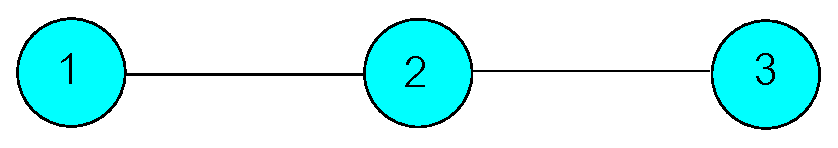
\includegraphics[width=3in]{figure/3nodes-chain}
\caption{A simple multi-hop network.}
\label{fig:3nodes-chain}
\end{figure}

\begin{figure}[!t]
\centering
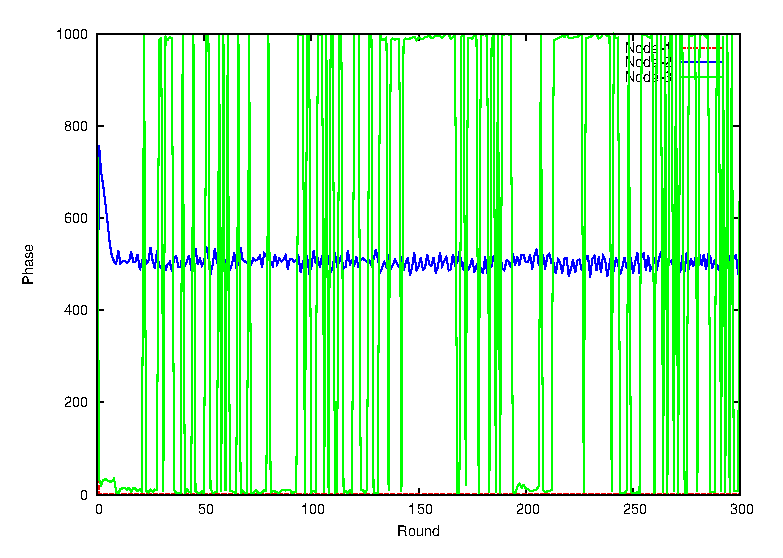
\includegraphics[width=3.5in]{figure/3nodes-chain-dwarf}
\caption{Message collision on a 3-node multi-hop chain network. The period T is 1000 milliseconds. Node 1 is at phase 0 whereas node 3 is approximately at the same phase as node 1.}
\label{fig:3nodes-chain-dwarf}
\end{figure}

\begin{figure}[!t]
\centering
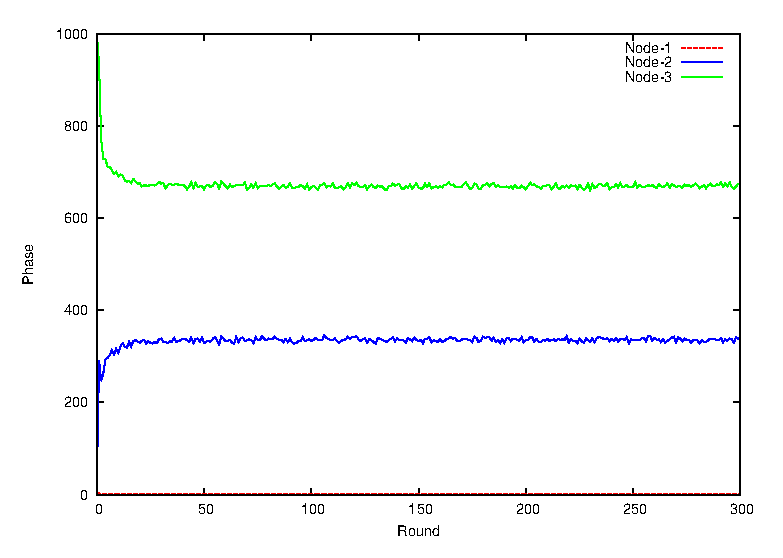
\includegraphics[width=3.5in]{figure/3nodes-chain-expected}
\caption{The perfect desynchrony state of a 3-node multi-hop chain network, The period T is 1000 milliseconds. Node 1 is at phase 0 whereas others are separated by T/3 milliseconds.}
\label{fig:3nodes-chain-expected}
\end{figure}

We have simulated DWARF by setting the period to 1000 milliseconds. Nodes wake up randomly. 
The simulation result is shown in Figure \ref{fig:3nodes-chain-dwarf}. Node 2's and node 3's phases are plotted relatively to the node 1's phase (\textit{i.e.}, the node 1's phase is relatively plotted to itself at 0). The noisy vertical line is the wrapping-around phase of node 3. The result shows that node 1 and node 3 fire messages approximately at the same phase. This causes the message collision at node 2.
However, the expected result (\textit{i.e.} perfect desynchrony state) should be that three nodes are separated equivalently because all nodes will interfere each other if they fire messages at the same phase. The expected result is shown in Figure \ref{fig:3nodes-chain-expected} where each node is equivalently separated from each other approximately by 1000/3 milliseconds.

The problematic result is caused by the hidden terminal problem as demonstrated in Figure \ref{fig:3nodes-chain-hidden}; node 1 and node 3 are hidden to each other in this multi-hop topology. While node 3 is firing a message, node 1 senses a wireless channel and does not detect any signal from node 3 because the signal from node 3 is not strong enough within the signal sensing range of node 1 and vice versa. Therefore, in DWARF, node 1 and node 3 notice only that there are two nodes, which are itself and node 2, in their perceived networks. Therefore, node 1 and node 3 simultaneously attempt to adjust their phases to the opposite side of node 2 in their time circles which are the same phase. As a result, their firing messages collide at node 2. 

\begin{figure}[!t]
\centering
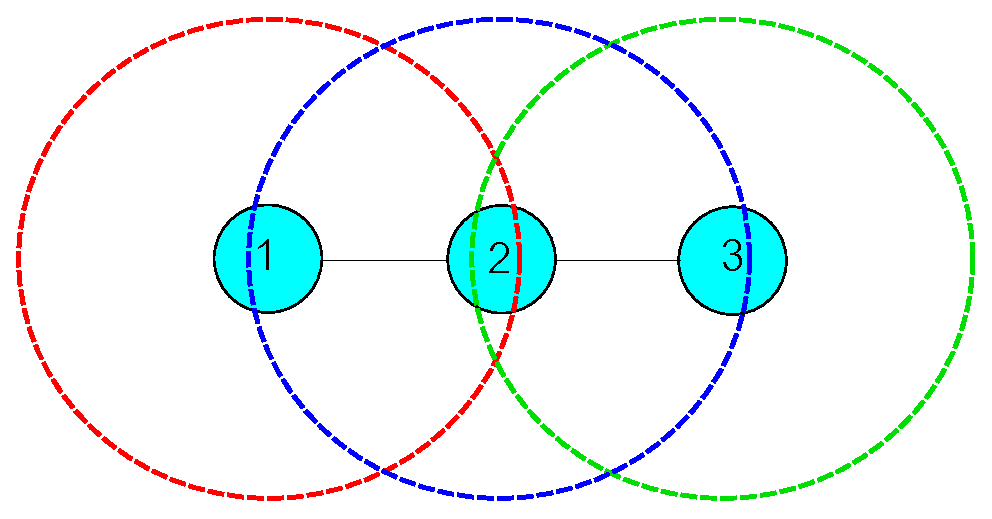
\includegraphics[width=4in]{figure/3nodes-chain-hidden}
\caption{The hidden terminal problem.}
\label{fig:3nodes-chain-hidden}
\end{figure}

The hidden terminal problem does not only affect the performance of DWARF but also affect that of DESYNC.
This is due to the fact that, in DESYNC, a node adjusts its phase based on firing messages from its perceived phase neighbors. In \cite{4663417} and \cite{MK09DESYNC}, EXTENDED-DESYNC, which is the extension of DESYNC, is proposed to solve the hidden terminal problem based on a relative time relaying mechanism. Based on the similar idea, we extend DWARF to support multi-hop topologies.
However, only relative time relaying mechanism does not lead DWARF to an optimal solution in some cases. Therefore, this dissertation also proposes a \textit{force absorption} mechanism for extending DWARF to support multi-hop networks.   

\section{DWARF with Multi-hop Extension (M-DWARF)}
\label{sec:extension}
\subsection{Relative Time Relaying}
\label{sec:relative}
The first idea to solve the hidden terminal problem is straightforward. If a node does not know the firing times of its second-hop neighbors, its one-hop neighbors relay such information. Therefore, instead of firing only to notify its firing time, each node includes their one-hop neighbors' firing times into a firing message. 

However, due to our assumption that nodes' clocks are not synchronized, relying on second-hop neighbors' firing timestamps from its one-hop neighbors could lead to wrong phase adjustment. This problematic scenario is demonstrated in Figure \ref{fig:broadcast-problem}. Figure \ref{fig:broadcast-problem-topo} illustrates the firing message of node 2 that contains timestamps of its one-hop neighbors. Figure \ref{fig:broadcast-problem-ring} shows the problem. The inner circle represents the local time of node 1 and the outer circle represents the local time of node 2. The figure indicates that the local reference times (at 0 millisecond) of node 1 and node 2 are different. Therefore, if node 1 uses the node 3's firing time relayed by node 2, which is 125 milliseconds, node 1 will misunderstand the exact time phase of node 3. The misunderstood phase of node 3 is depicted as a dash circle. 

\begin{figure*}[!t]
\centerline{
	\subfloat[]{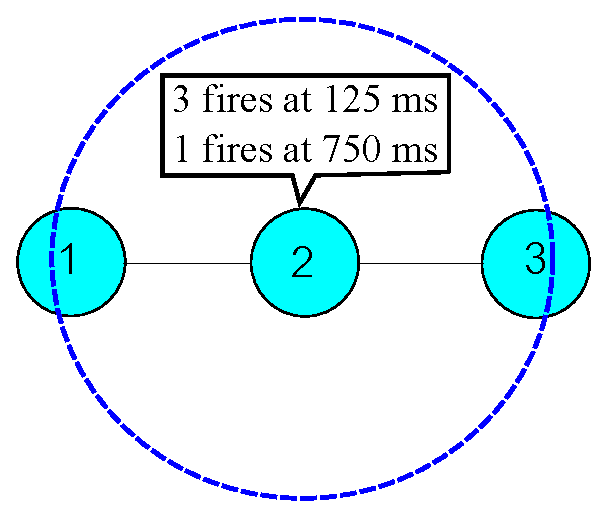
\includegraphics[scale=0.60]{figure/broadcast-problem-topo}%
	\label{fig:broadcast-problem-topo}}
	\hfil
	\subfloat[]{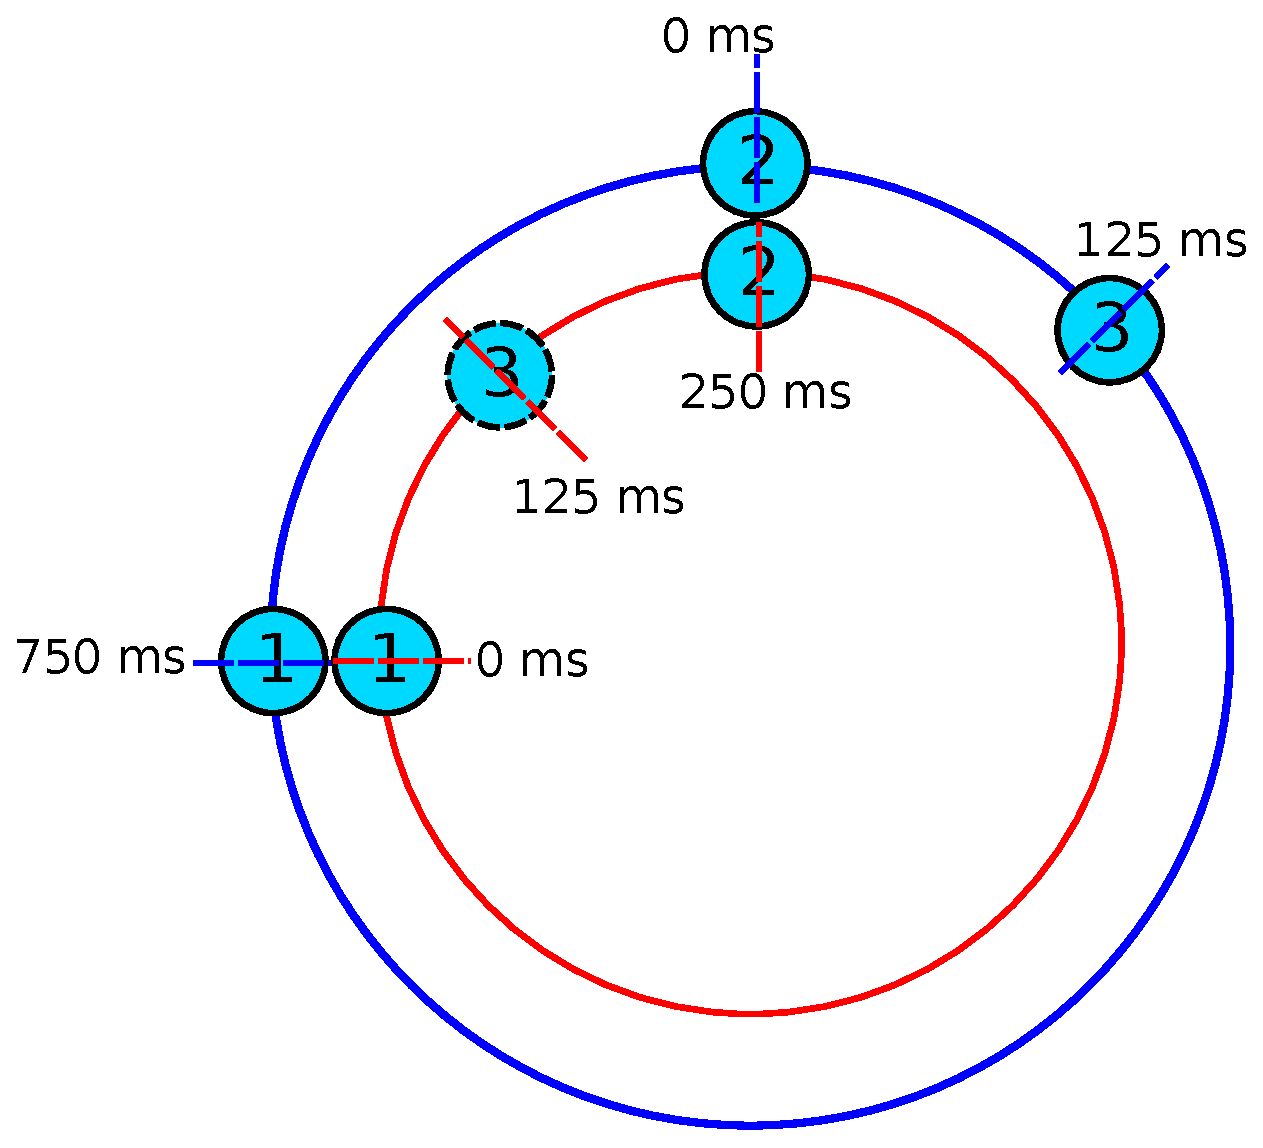
\includegraphics[scale=0.35]{figure/broadcast-problem-ring}%
	\label{fig:broadcast-problem-ring}}
}
\caption{A node includes its one-hop neighbors' firing times into a firing message. (a) Node 2 fires a message containing node 1's and node 2's firing timestamps that it perceives. (b) Node 1 misunderstands the time phase of node 3 because local time of node 1 and local time of node 2 are different.}
\label{fig:broadcast-problem}
\lofcont
\end{figure*}

This problem can be simply solved by using relative phases instead of actual local times. Each node fires a message that includes relative phases of its one-hop neighbors. A receiving node marks the firing phase of the firing node as a reference phase. Then, the receiving node perceives its second-hop neighbors' phases as relative phases offset by the reference phase. Figure \ref{fig:broadcast-relative} shows how extended DWARF desynchronizes a 3-node multi-hop chain network.

\begin{figure*}[!t]
\centerline{
	\subfloat[]{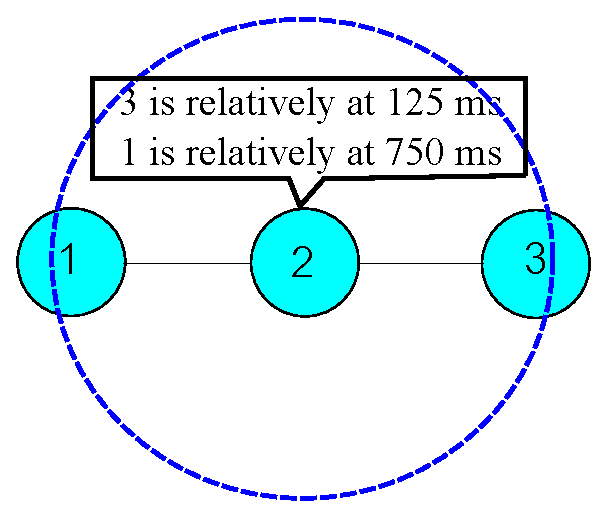
\includegraphics[scale=0.45]{figure/broadcast-relative-topo}%
	\label{fig:broadcast-relative-topo}}
	\hfil
	\subfloat[]{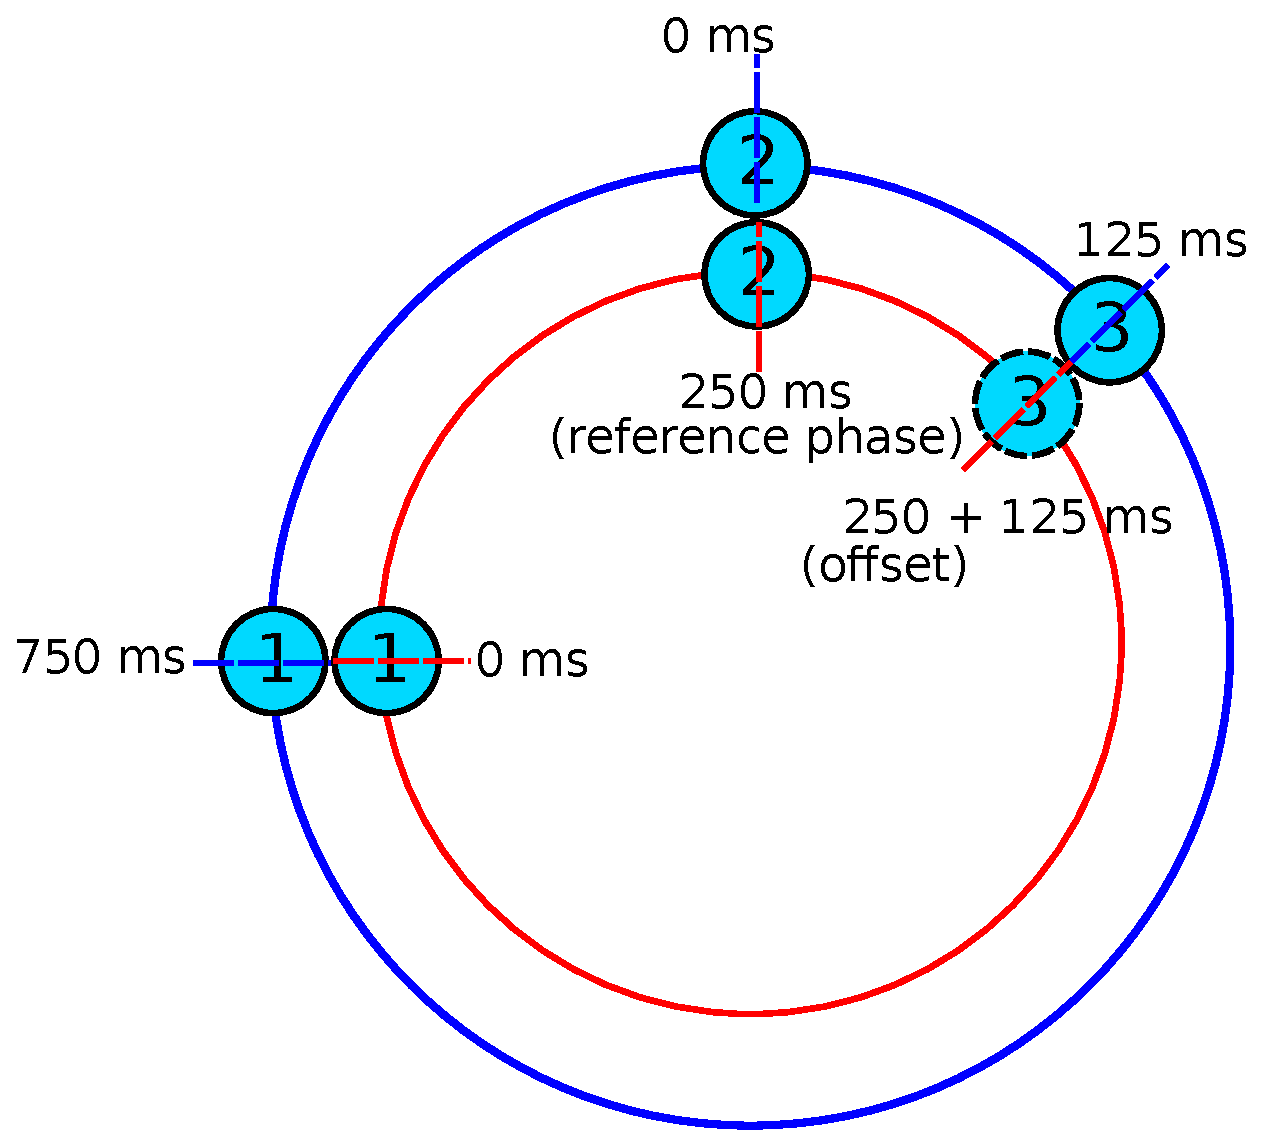
\includegraphics[scale=0.25]{figure/broadcast-relative-ring}%
	\label{fig:broadcast-relative-ring}}
	\hfil
	\subfloat[]{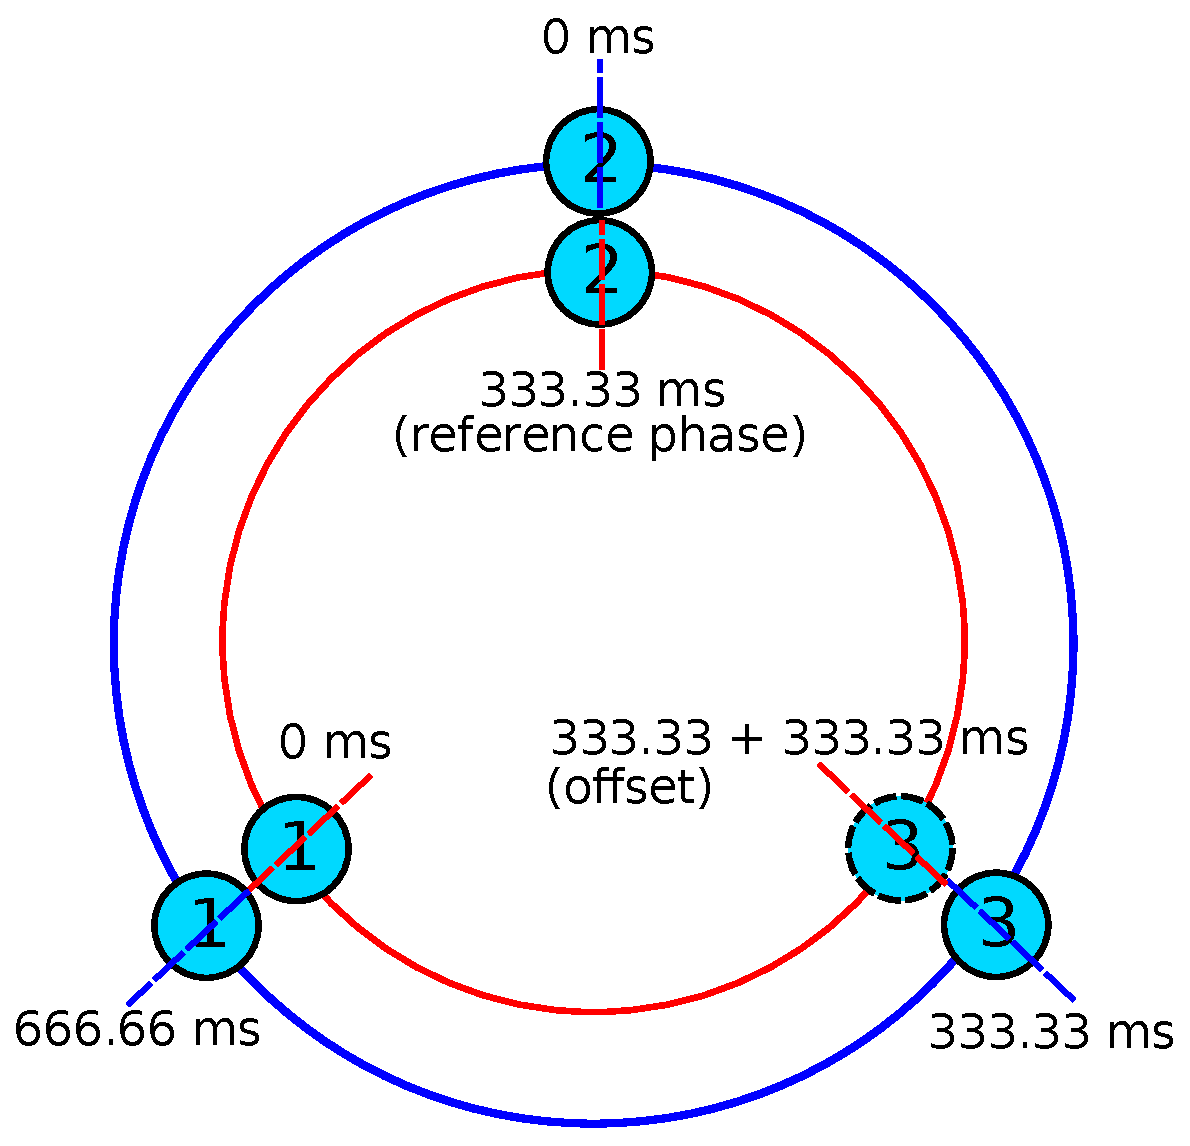
\includegraphics[scale=0.25]{figure/broadcast-relative-perfect}%
	\label{fig:broadcast-relative-perfect}}
}
\caption{EXT-DWARF: A node includes its one-hop neighbors' relative phases into a firing message. (a) Node 2 fires a message containing node 1's and node 2's relative phases. (b) Node 1 marks the node 2's phase as a reference phase and uses it as an offset for calculating the node 3's phase. (c) Eventually, nodes are in the perfect desynchrony state.}
\label{fig:broadcast-relative}
\lofcont
\end{figure*}


\subsection{Force Absorption}
\label{sec:absorption}
As we mentioned earlier, DWARF with the relative time relaying mechanism does not solve some cases.
These cases are when there are at least two second-hop neighbors that can share the same phase without interference. For example, in a 4-node chain network illustrated in Figure \ref{fig:4nodes-chain-topo}, node 2 and node 3 are physically far beyond two hops. Therefore, they can fire messages at the same time phase as shown in Figure \ref{fig:4nodes-chain-expected}.
However, in extended DWARF, node 0 perceives that node 2 and node 3 are at the same phase. Therefore, there are two forces from node 2 and node 3 to repel node 0 forward but there is only force from node 1 to repel node 0 backward. Consequently, node 0 cannot stay at the middle between node 1 and the group of node 2 and 3 (see Figure \ref{fig:4nodes-chain-dwarf}). 

\begin{figure*}[!t]
\centerline{
	\subfloat[]{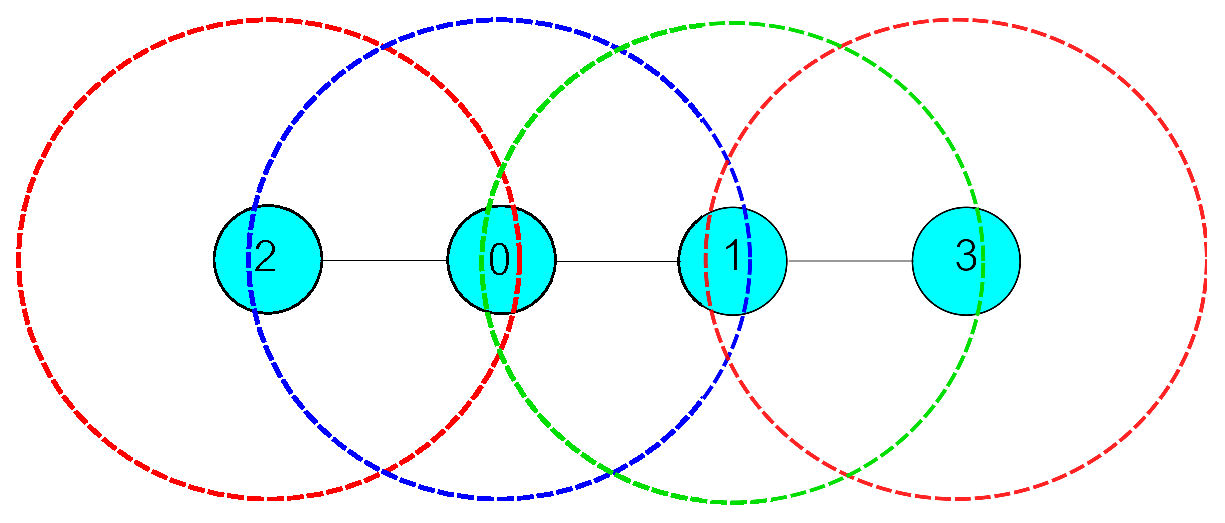
\includegraphics[scale=0.3]{figure/4nodes-chain-topo}%
	\label{fig:4nodes-chain-topo}}
	\hfill
	\subfloat[]{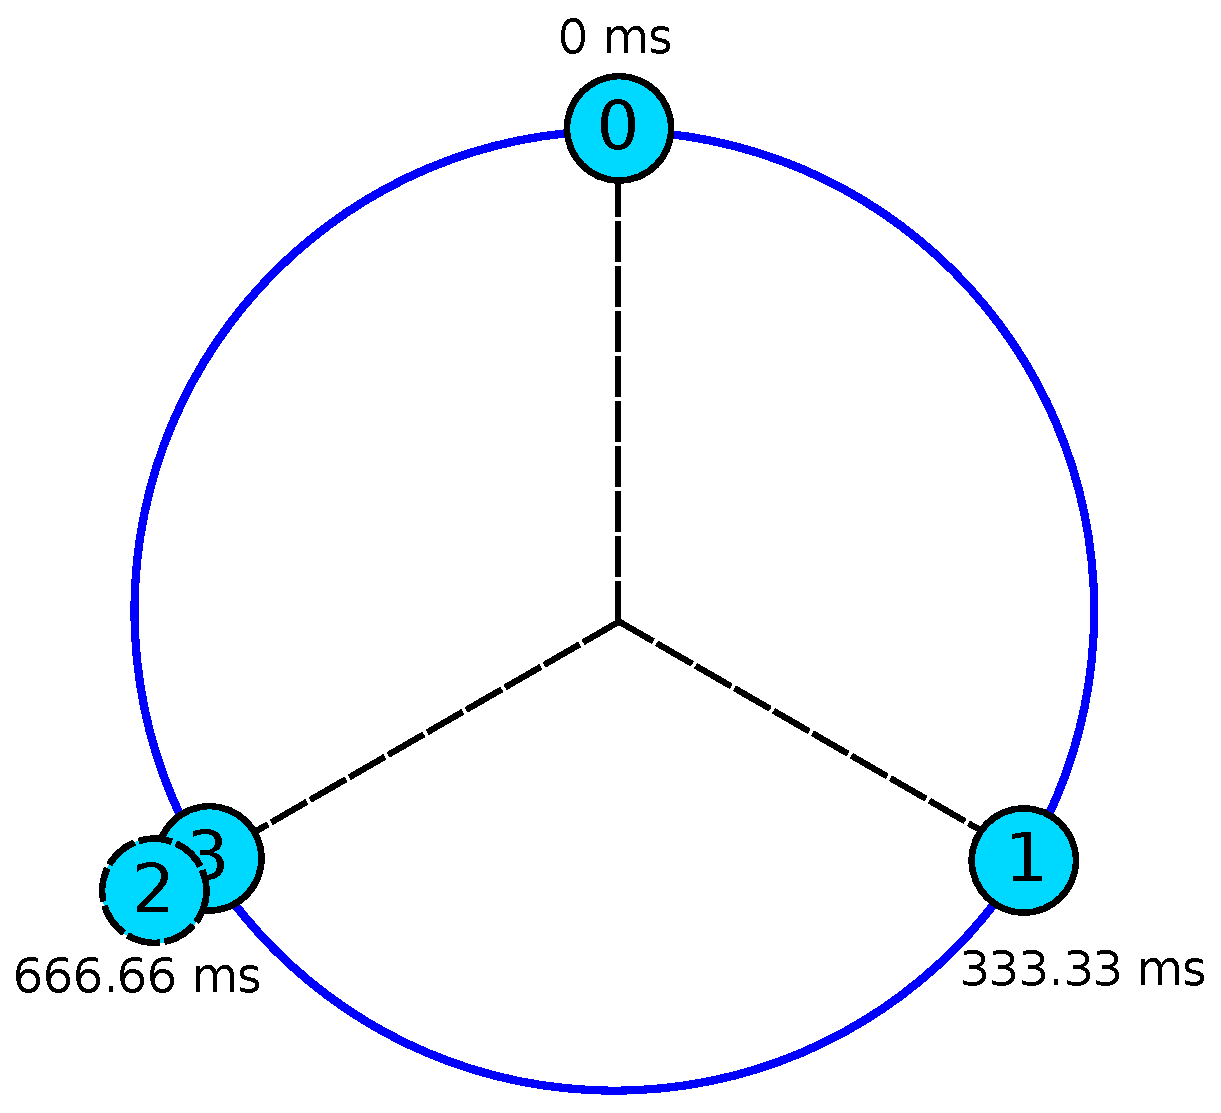
\includegraphics[scale=0.20]{figure/4nodes-chain-expected}%
	\label{fig:4nodes-chain-expected}}
	\hfill
	\subfloat[]{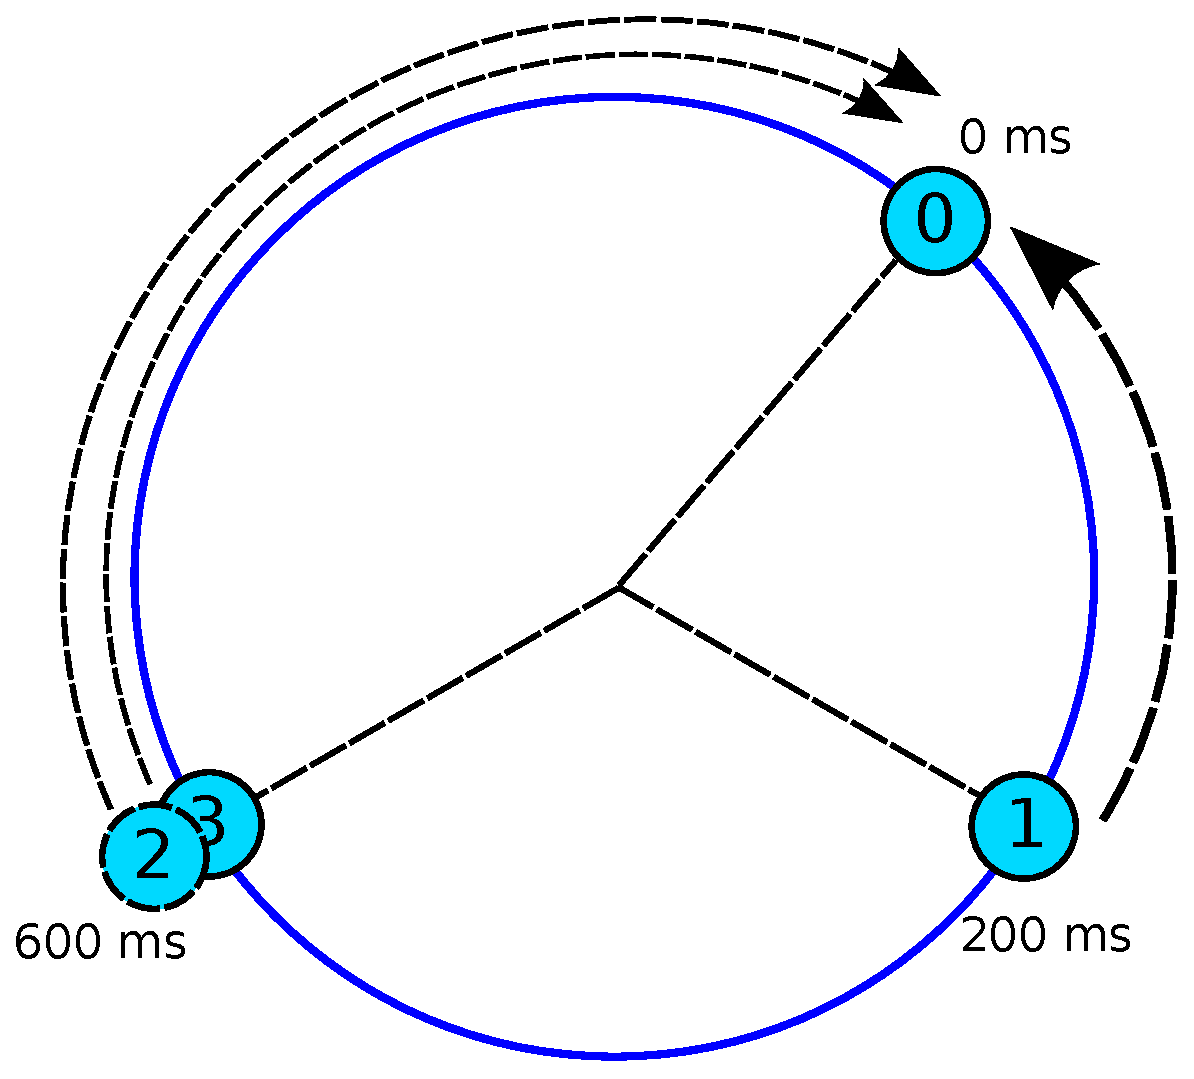
\includegraphics[scale=0.20]{figure/4nodes-chain-dwarf}%
	\label{fig:4nodes-chain-dwarf}}
}
\caption{The problem of the single-hop DWARF algorithm. (a) A 4-node chain topology. The transmission signal of node 2 does not interfere any receiver of node 3 and vice versa. (b) In the node 0's local view, the expected result is that node 2 and node 3 can share the same phase without interference. (c) In extended DWARF, node 0 is not in the expected phase because there are two forward repelling forces from node 2 and node 3 while there is one backward repelling force from node 1.}
\label{fig:4nodes-chain}
\lofcont
\end{figure*}

Therefore, we propose a novel force absorption mechanism for multi-hop desynchronization based on the artificial force field.
The objective of this mechanism is to absorb the overwhelming force from at least two nodes that can fire at the same phase without interference.

The mechanism is as follows. A node receives a full repelling force from the next/previous phase neighbor as in DWARF. However, a force from the second-next/second-previous phase neighbor is partially absorbed by the next/previous phase neighbor. The magnitude of the absorbed force depends on the phase interval between the next/previous and the second-next/second-previous phase neighbors.  The closer that the second-next/second-previous phase neighbor moves to the next/previous phase neighbor results in the lower magnitude of the absorbed force. Eventually, when the second-next/second-previous phase neighbor moves to the same phase as the next/previous phase neighbor, the additional force from the second-next/second-previous phase neighbor is fully absorbed. Consequently, the magnitude of two forces repelling the considered node is approximately equal to only magnitude of one force. This principle is applied recursively; the force from the third-next/third-previous phase neighbor is absorbed by the second-next/second-previous phase neighbor, the force from the fourth-next/fourth-previous phase neighbor is absorbed by the third-next/third-previous phase neighbor, and so forth.   
Figure \ref{fig:4nodes-chain-dwarf-absorb} illustrates this mechanism. In Figure \ref{fig:4nodes-chain-dwarf-absorb-split}, the force from node 2 to node 0 is absorbed by node 3 (the absorbed force is displayed in a blur line). Thus, from node 2, there is only small magnitude of force left to node 0. Eventually, in Figure \ref{fig:4nodes-chain-dwarf-absorb-perfect}, node 2 moves to the same phase as node 3 because they do not interfere each other and the force from node 2 is fully absorbed. Consequently, the network can be in the perfect desynchrony state.

\begin{figure*}[!t]
\centerline{
	\subfloat[]{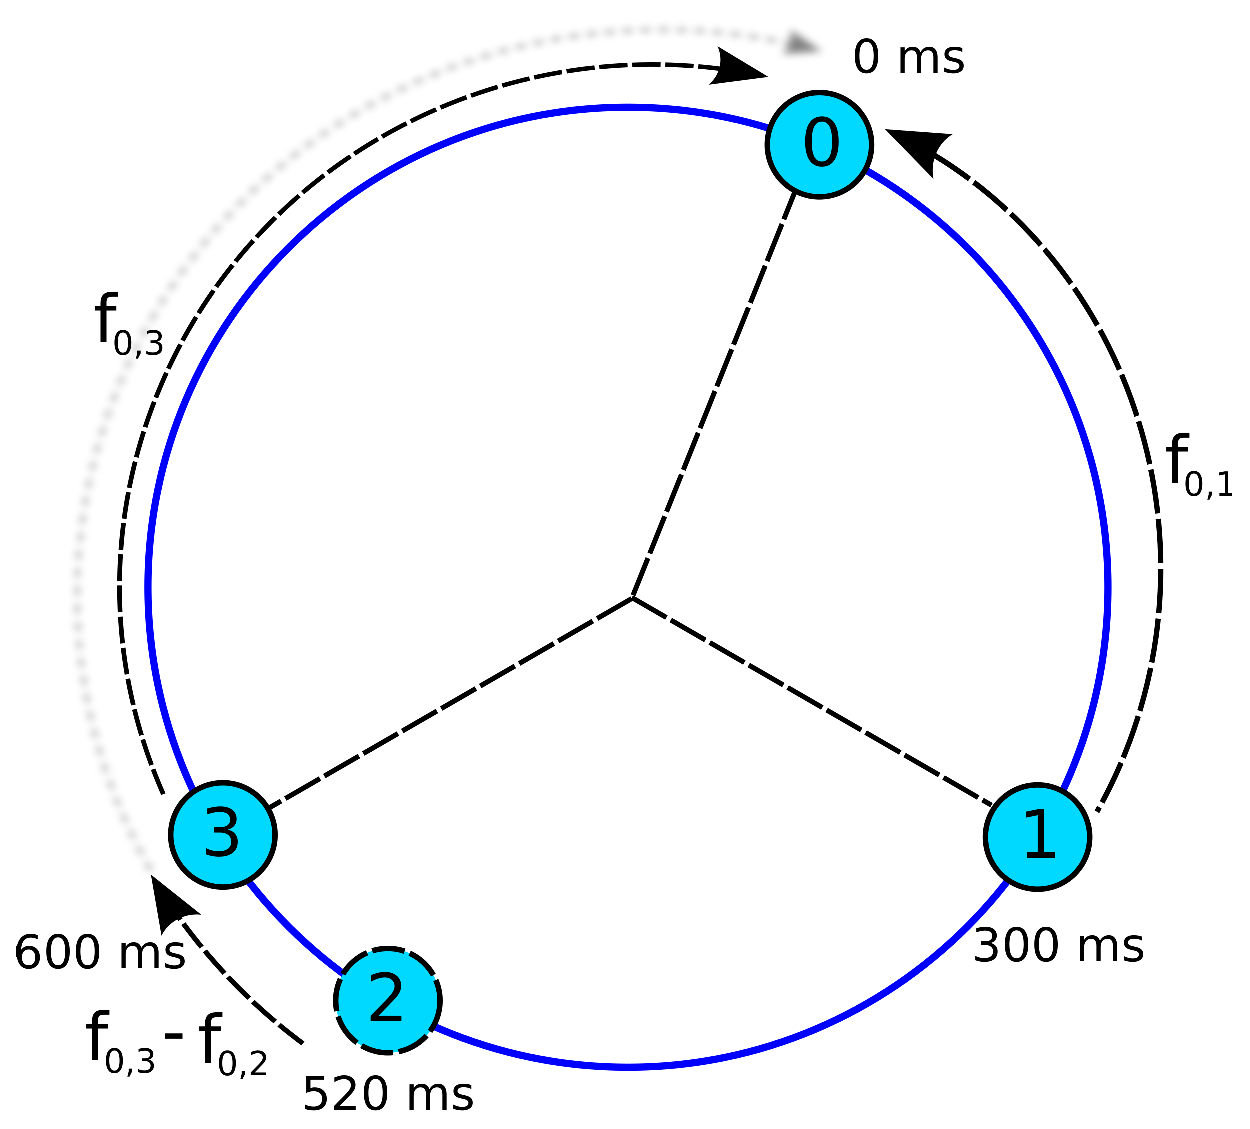
\includegraphics[scale=0.33]{figure/4nodes-chain-dwarf-absorb-split}%
	\label{fig:4nodes-chain-dwarf-absorb-split}}
	\hfil
	\subfloat[]{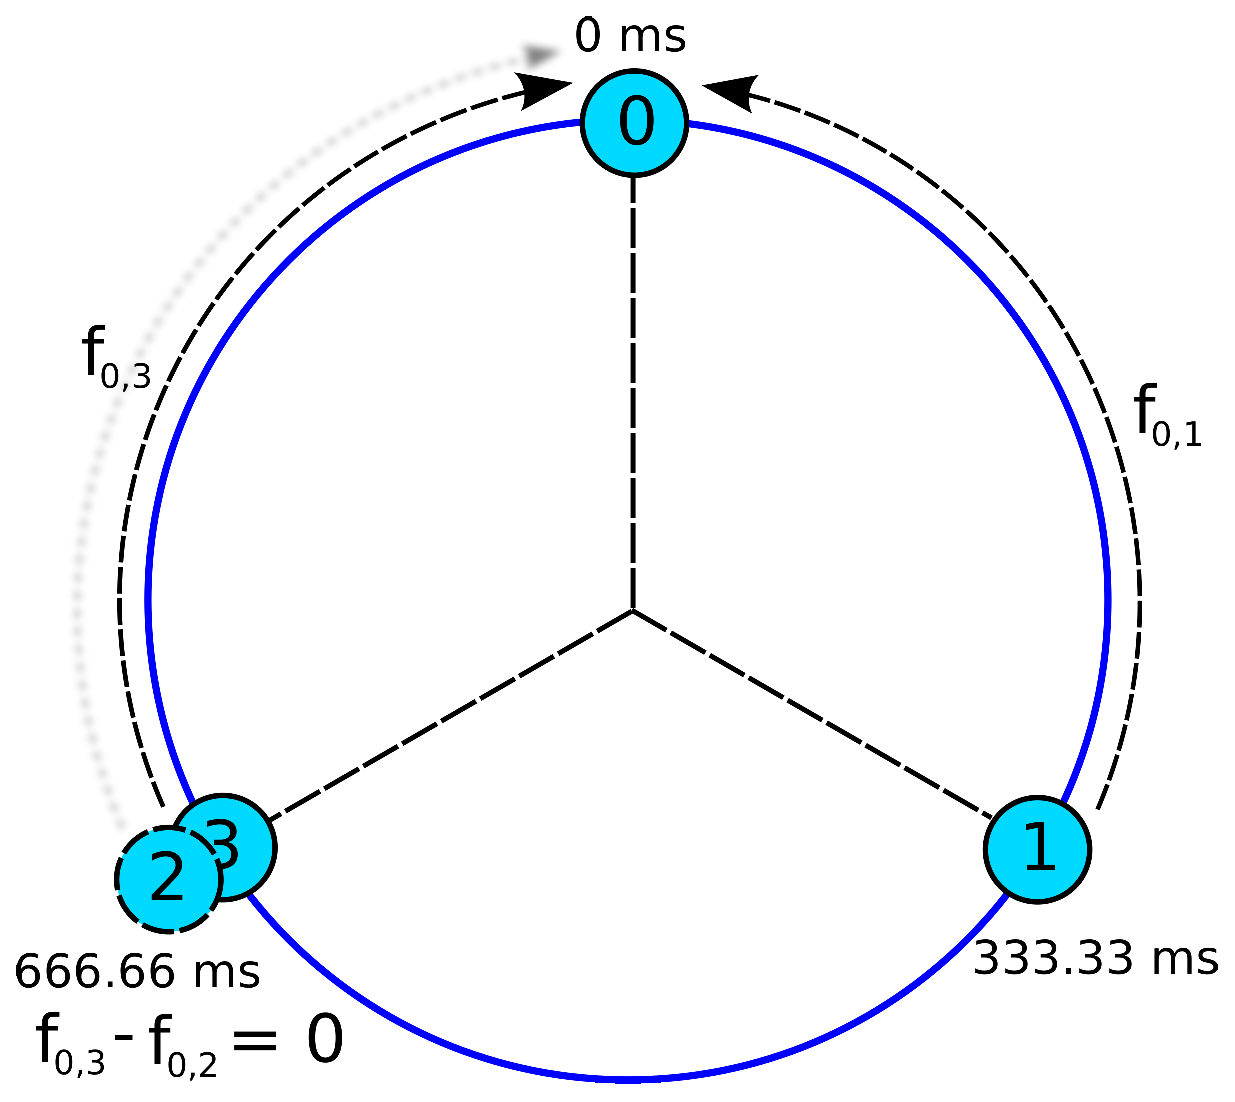
\includegraphics[scale=0.33]{figure/4nodes-chain-dwarf-absorb-perfect}%
	\label{fig:4nodes-chain-dwarf-absorb-perfect}}
}
\caption{EXT-DWARF with force absorption. The blur line represented an absorbed force. (a) When node 2 and 3 are apart, the force from node 2 affects node 0 but the force is partly absorbed. (b) When node 2 and 3 are at the same phase, the force from node 2 is fully absorbed.}
\label{fig:4nodes-chain-dwarf-absorb}
\lofcont
\end{figure*}

Let $f_{i,j}$ be a full repelling force from node $j$ to node $i$, $f_{i,j}^{'}$ be an absorbed force from node $j$ to node $i$, $T$ is the time period, and $\Delta \phi_{i,j}$ is the phase difference between node $i$ and $j$. 
The force function for multi-hop networks is the following:
\begin{alignat}{2}
f_{i,j} &= \frac{1}{\Delta \phi_{i,j} / T}, \text{where }\Delta \phi_{i,j} \in (-\frac{T}{2}, \frac{T}{2}) \nonumber \\
f_{i,i + 1}^{'} &= f_{i,i + 1} \nonumber \\
f_{i, i - 1}^{'} &= f_{i,i - 1} \nonumber \\
f_{i,j}^{'} &= f_{i,x} - f_{i,j}, \text{where } j \notin \left\{i -1, i + 1\right\} \text{ and } x = (j - \frac{\Delta \phi_{i,j}}{|\Delta \phi_{i,j}|}) \mod n.
\label{eq:force-absorb}
\end{alignat}
For $f_{i,x}$, if node $j$ repels node $i$ forward, $x$ is $j + 1$. In contrast, if node $j$ repels node $i$ backward, $x$ is $j - 1$. At $T/2$ or $-T/2$, a node does not repel an opposite node because they are balanced.

For example, in Figure \ref{fig:4nodes-chain-dwarf-absorb}, node 0 calculates the force from node 2 as the following:
\begin{alignat}{2}
f_{0,2}^{'} &= f_{0,3} - f_{0,2} \nonumber \\
&= \frac{1}{\Delta \phi_{0,3} / T} - \frac{1}{\Delta \phi_{0,2} / T}. \nonumber
\end{alignat} 

Noticeably, if node 2 moves close to node 3, the value of $\Delta \phi_{0,2}$ is close to the value of $\Delta \phi_{0,3}$. Then, the magnitude of force $f_{0,2}$ is reduced. 
Finally, when $\Delta \phi_{0,2}$ is equal to $\Delta \phi_{0,3}$ as in Figure \ref{fig:4nodes-chain-dwarf-absorb-perfect}, the magnitude of force $f_{0,2}$ becomes 0. In other words, the force is fully absorbed. 

\section{M-DWARF Algorithm}
\label{sec:multihop-algo}
The M-DWARF algorithm is similar to DWARF (see Chapter \ref{chap:algo}). However, M-DWARF has two proposed mechanisms to support multi-hop topologies: relative time relaying and force absorption. Initially, nodes are not desynchronized. 
Each node sets a timer to fire in $T$ time unit and listens to all one-hop neighbors.

When receiving a firing message from its one-hop neighbor, the receiving node marks the current time to be the relative phase reference. Then, the node reads relative phases of its two-hop neighbors which are included within the firing message. After that, the node calculates their two-hop neighbors' phases by using the relative phase reference as the offset.  

When the timer expires, the node broadcasts a firing message containing relative phases of its one-hop neighbors. 
Then, the node calculates a new time phase to move on the phase circle. The calculation is based on the summation of artificial forces from all phase neighbors within two-hops where some forces are absorbed. Then, the node sets a new timer according to the new calculated phase.

As same as DWARF, a node adjusts its phase as follows.
Given the total received absorbed force $\mathcal{F}_i$, the node $i$ adjusts to a new time phase $\phi_i^{'}$,
\begin{equation}
\phi_i^{'} = (\phi_i + K\mathcal{F}_i) \mod T,
\label{eq:newphase-mhop}
\end{equation} 
where $\phi_i$ is the current phase of the node $i$.

We choose the coefficient $K$ as same as in DWARF: 
\begin{equation}
K = 38.597 \times n^{-1.874} \times \frac{T}{1000},
\end{equation}
where $n$ is the number of phase neighbors within two hops and $T$ is the time period.
We refer to Section \ref{sec:algo} that proves and describes in details how we get the value of the coefficient $K$. In short, the value of the coefficient $K$ is inverse proportional to the number of nodes $n$ and proportional to the time period $T$.

All nodes in the artificial force field (in the period circle) iteratively run the same algorithm until the force is balanced.
The pseudo-code of this algorithm is shown in Figure \ref{fig:pseudocodemdwarf}.


\begin{figure}[!t]
\begin{algorithmic}[1]
	\STATE \textbf{Initialization}  
  	\STATE $T = TimePeriod$ \COMMENT{Configurable Time Period}
  	\STATE $n = 1$ \COMMENT{Number of neighbors within two hops including itself}
  	\STATE $\mathcal{F} = 0$ \COMMENT{Force Summation}
  	\STATE $phasesBuffer = Array$ \COMMENT{Buffer for phases of neighbors within two hops}
  	\STATE $lastFiringTime = localTime$
  	\STATE $currentPhase = localTime$ modulo $T$
  	\STATE Set a firing timer to be $T$ unit time
  	\newline
  	
  	\STATE \textbf{Upon timer firing}
    \STATE Broadcast a firing message containing relative phases of one-hop neighbors
    \STATE $lastFiringTime = localTime$
  	\STATE $currentPhase= localTime$ modulo $T$
    \STATE $K = 38.597 \times n^{-1.874} \times \frac{T}{1000}$
    \STATE $\mathcal{F}$ = call Calculate total force
    \STATE $newPhase = currentPhase + (K \times \mathcal{F})$
    \IF{$newPhase < 0$}
    	\STATE $newPhase = T + newPhase$
	\ENDIF
    \STATE Set a firing timer to be fired at ($newPhase$ modulo $T$)
   	\STATE $\mathcal{F} = 0$
   	\STATE $n = 1$
 	\newline
 	
 	\STATE \textbf{Calculate total force}
 	\STATE $sortedBuffer$ = Sort $phasesBuffer$
 	\STATE $forwardForce = \frac{1}{(T - sortedBuffer[length - 1])/T}$
 	\STATE $backwardForce = \frac{1}{sortedBuffer[0]/T}$
    \FOR{$i$ in range of 1 to length of sorted $phasesBuffer$ - 2}
      \IF{$phasesBuffer[i] > 0.5T$}
        \STATE $forwardForce = forwardForce + (\frac{1}{(T - phasesBuffer[i+1]) / T} - \frac{1}{(T - phasesBuffer[i]) / T})$
      \ELSE
        \STATE $backwardForce = backwardForce + (\frac{1}{phaseBuffer[i-1] / T} - \frac{1}{phaseBuffer[i] / T})$
      \ENDIF
    \ENDFOR
    \STATE return $forwardForce - backwardForce$
 	\newline
 	   
    \STATE \textbf{Upon receiving a firing message from $nodeId$}
    \STATE $phaseDiff = localTime - lastFiringTime$
    \STATE $phasesBuffer[nodeId] = phaseDiff$
    \STATE $reference = phaseDiff$
    \FOR{each $twoHopNodeId$ of two-hop neighbors in $message$}
      \IF{$twoHopNodeId$ is not in $phasesBuffer$} 
        \STATE $phasesBuffer[twoHopNodeId] = message[twoHopNodeId][relativePhase] + reference$
        \STATE $n = n + 1$
      \ENDIF
    \ENDFOR
\end{algorithmic}
\caption{Pseudocode of M-DWARF algorithm}
\label{fig:pseudocodemdwarf}
\end{figure}

\section{Evaluation}
\label{sec:multihop-evaluation}
In this section, we evaluate the performance of M-DWARF, EXTENDED-DESYNC (\cite{MK09DESYNC}), and LIGHTWEIGHT (\cite{5062165}). All of these algorithms do not require time synchronization. We begin by measuring the desynchronization error and convergence time on single-hop networks because the extension for multi-hop networks should work on single-hop networks as well. Then, we evaluate on several multi-hop topologies which are used in the previous work (\cite{4663417}).

\subsection{Evaluation Environment}
We implement M-DWARF, EXTENDED-DESYNC, and LIGHTWEIGHT on Tiny-OS 2.1.2 and evaluate them on the TOSSIM simulator.
In our simulation, for all algorithms, we use 2-byte sender node ID, and 2-byte neighbor ID. For M-DWARF and EXTENDED-DESYNC, we use 2-byte relative phase for each one-hop neighbor. The regular 11-byte CC2420 header is also used.
The time period is set to 1000, 2000, and 3000 milliseconds.
The step size ($\alpha$) of EXTENDED-DESYNC is set to 0.95 as same as in Chapter \ref{chap:algo}.
The phase of each node is initially random in a range of 0 to the period length 


\subsection{Single-hop Networks (Fully-connected Topology) Evaluation}
We begin by evaluating M-DWARF on single-hop networks. In M-DWARF and EXTENDED-DESYNC, each firing message contains relative phases of one-hop neighbors. Therefore, to limit the size of a message, we vary the one-hop network size from 4 to 32 nodes.

\subsubsection{Desynchronization Error}
We run the simulation for 300 time periods to measure the desynchronization error. 
In each network size, we run the simulation for 30 times.
Then, we measure the average root mean square error (RMSE) and normalized root mean square error (see details in Section \ref{sec:error}). 
Figure  \ref{fig:rmse300rounds-mhop} illustrates the result of absolute desynchronization error and Figure \ref{fig:nrmse300rounds-mhop} illustrates the result of the normalized desynchronization error in each network size after 300 time periods.

\begin{figure*}[!t]
\centerline {
	\subfloat[]{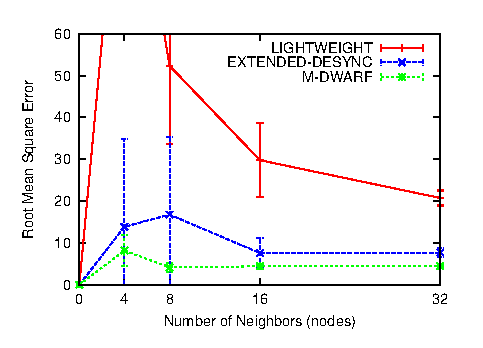
\includegraphics[width=3.0in]{figure/compare300rounds_rmse_sd_mhop}%
	\label{fig:rmse300rounds-mhop}}
	\hfil
	\subfloat[]{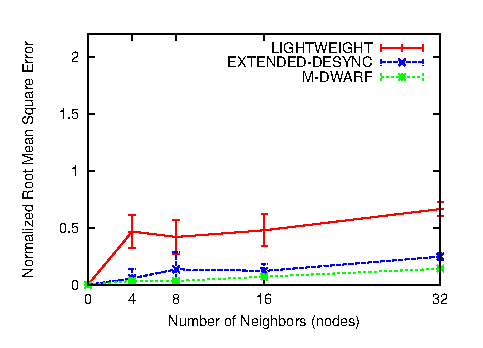
\includegraphics[width=3.0in]{figure/compare300rounds_nrmse-expected_sd_mhop}%
	\label{fig:nrmse300rounds-mhop}}
}
\caption{(a) Root mean square error after 300 time periods. (b) Root mean square error normalized by perfect phase difference after 300 time periods.}
\lofcont
\end{figure*}

The result indicates that, in all network sizes (4 - 32 nodes), M-DWARF achieves significantly better desynchrony states than EXTENDED-DESYNC and LIGHTWEIGHT do. 
The EXTENDED-DESYNC's mechanism has the same pitfall as that of DESYNC because they are based on the same mechanism. The pitfall is that the phase error of a node propagates to its phase neighbors and this error will propagate back and forth between two phase neighbors. This results in a large error after convergence.
In contrast, M-DWARF is robust to this error propagation as same as DWARF because both M-DWARF and DWARF use the total received forces from all neighbors. An error from one neighbor does not overwhelm the system.
For LIGHTWEIGHT, the desynchronization errors of small networks are extremely large because the algorithm randomly chooses the free time slot without considering the equitably separation. However, when the network size becomes larger, the error becomes lower because the perfect phase interval length is reduced.

\begin{figure*}[!t]
\centerline{
	\subfloat[Sparse]{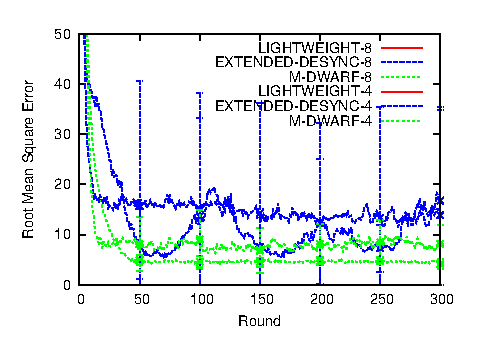
\includegraphics[width=3.0in]{figure/compare-rmse-4-8nodes_sd_mhop}%
	\label{fig:rmse-sparse-mhop}}
	\hfil
	\subfloat[Dense]{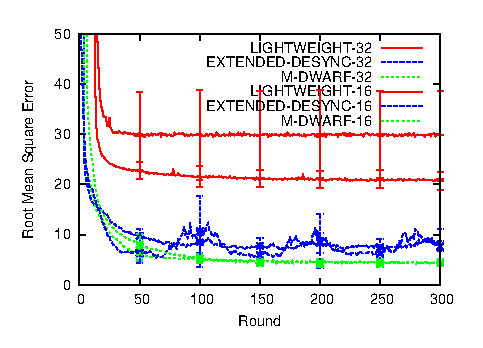
\includegraphics[width=3.0in]{figure/compare-rmse-16-32nodes_sd_mhop}%
	\label{fig:rmse-dense-mhop}}
}
\caption{Convergence time and absolute root mean square error}
\label{fig:rmse-convergence-mhop}
\lofcont
\end{figure*}

\begin{figure*}[!t]
\centerline{
	\subfloat[Sparse]{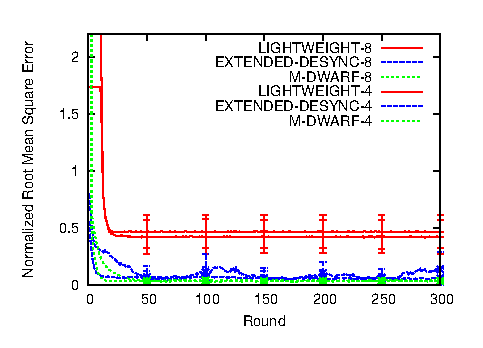
\includegraphics[width=3.0in]{figure/compare-nrmse-4-8nodes_sd_mhop}%
	\label{fig:nrmse-sparse-mhop}}
	\hfil
	\subfloat[Dense]{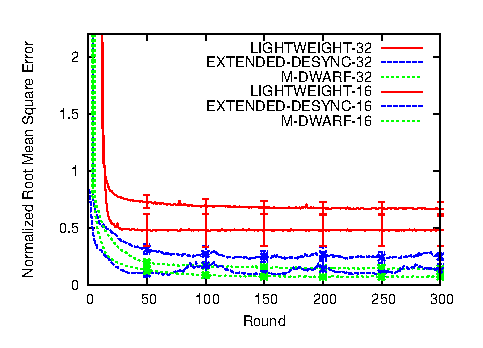
\includegraphics[width=3.0in]{figure/compare-nrmse-16-32nodes_sd_mhop}%
	\label{fig:nrmse-dense-mhop}}
}
\caption{Convergence time and root mean square error normalized by expected phase difference}
\label{fig:nrmse-convergence-mhop}
\lofcont
\end{figure*}

\subsubsection{Convergence Time}
\begin{figure*}
\centerline{
  \subfloat[8 nodes]{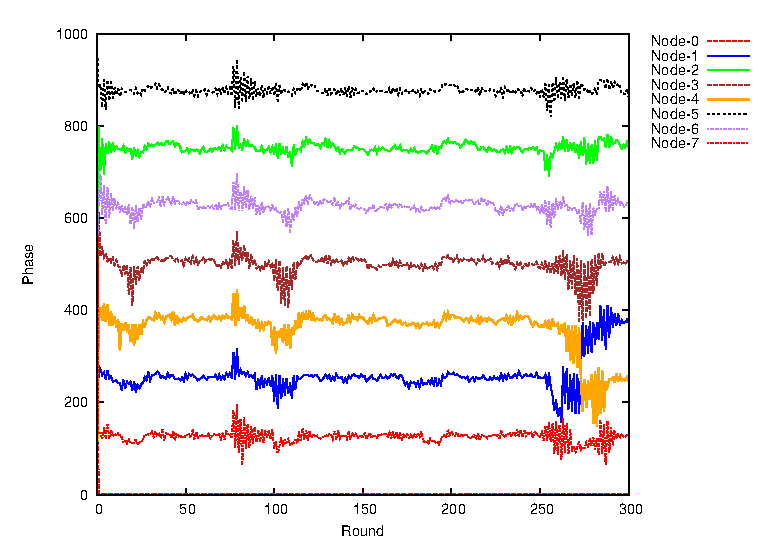
\includegraphics[scale=0.5]{figure/fluctuate-8}}
  \hfil
  \subfloat[16 nodes]{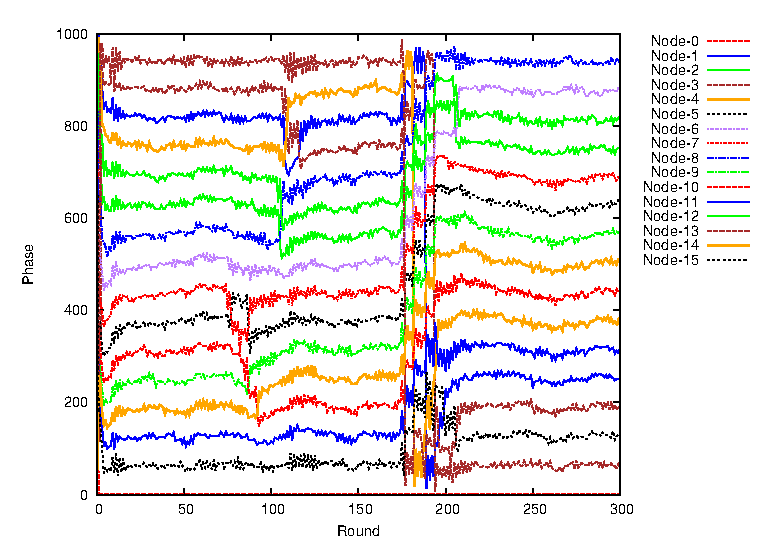
\includegraphics[scale=0.5]{figure/fluctuate-16}}
}
\caption{Fluctuation in some cases of EXTENDED-DESYNC.}
\label{fig:fluctuate}
\lofcont
\end{figure*}
In this section, we measure the absolute root mean square error and normalized root mean square error for each time period to investigate the convergence time.
Figure \ref{fig:rmse-sparse-mhop} and \ref{fig:nrmse-sparse-mhop} show the results of sparse networks whereas Figure \ref{fig:rmse-dense-mhop} and \ref{fig:nrmse-dense-mhop} show the results of dense networks.

In all network sizes, the convergence speed of M-DWARF is comparable to that of EXTENDED-DESYNC. However, M-DWARF converges with the lowest desynchronization error. For LIGHTWEIGHT, the algorithm converges fast and stable. However, due to the random slot selection process, the desynchronization errors in all network sizes are large.

We note that the errors of EXTENDED-DESYNC for 8-node and 16-node networks are fluctuate. This is due to the fact that, in our 30 EXTENDED-DESYNC simulations, there are some cases in 8-node and 16-node networks that the phases of some nodes are highly fluctuate as depicted in Figure \ref{fig:fluctuate}. These cases affect the average value. This behaviour is caused by the mechanism of EXTENDED-DESYNC (and DESYNC) that relies on only two phase neighbors information as described earlier in Chapter \ref{chap:algo}.

The result of single-hop networks indicates that M-DWARF that augments DWARF with two mechanisms still performs very well on single-hop networks without loss of generality. 


\subsection{Impact of Topologies}
For multi-hop networks, we evaluate M-DWARF on several topologies including star, chain, cycle, butterfly, and mesh topologies. In each topology, we simulate for 30 times and show the relative phase graph results. We show the phase graphs that represent the average case and the problematic case of each algorithm. We note that, in all topologies, LIGHTWEIGHT achieves the similar results. For LIGHTWEIGHT, each node randomly chooses the beginning of a time slot by avoiding the collision with one-hop neighbors. Therefore, on average, LIGHTWEIGHT causes several inequivalent interval gaps between two consecutive phase neighbor nodes. Moreover, there are several problematic cases that at least two nodes within two-hop communication choose the same beginning of a time slot because they cannot receive firing messages from each other. Thus, in all topologies, we only describe the behaviour of M-DWARF and EXTENDED-DESYNC.

\begin{figure*}[!t]
\centering{
	\subfloat[6 nodes]{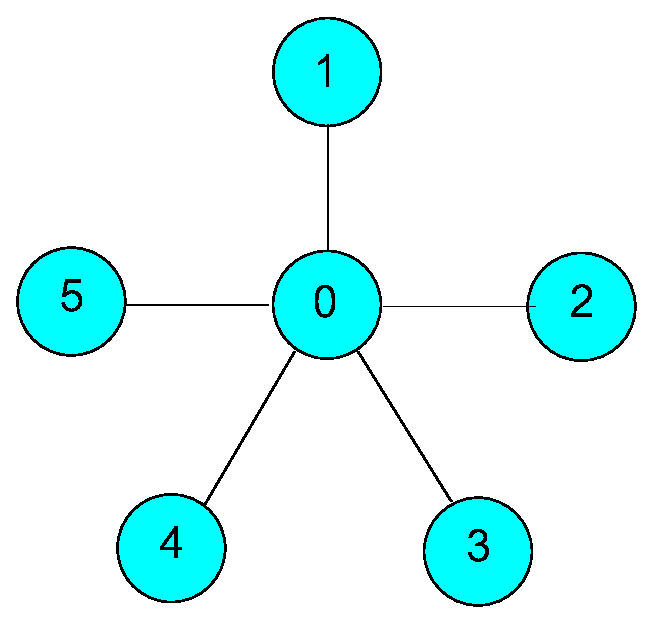
\includegraphics[scale=0.4]{figure/6nodes-star-eval}%
	\label{fig:6nodes-star-eval}}
	\hspace{1in}
	\subfloat[20 nodes]{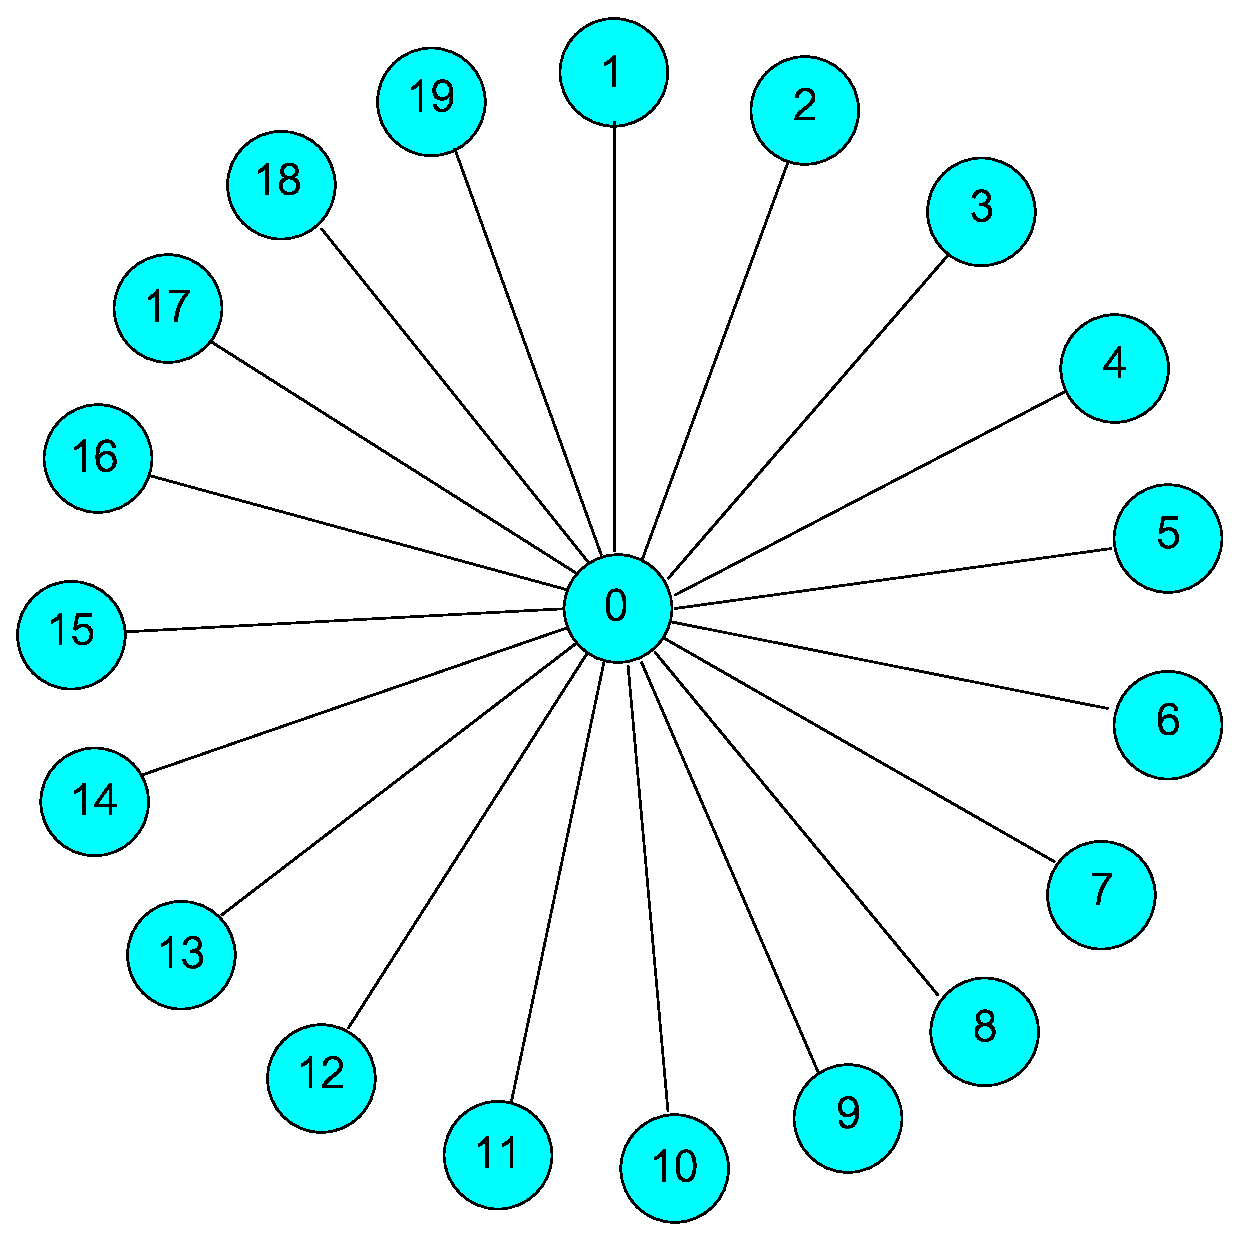
\includegraphics[scale=0.25]{figure/20nodes-star-eval}%
	\label{fig:20nodes-star-eval}}
}
\caption{Star topology}
\label{fig:star-eval}
\lofcont
\end{figure*}

\subsubsection{Star Topology}
\begin{figure*}[!t]
\centering{
	\subfloat[M-DWARF]{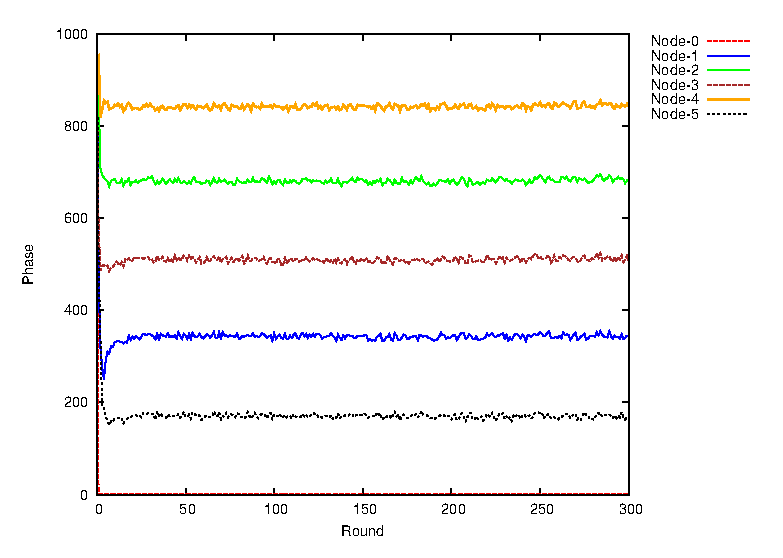
\includegraphics[scale=0.35]{figure/6nodes-star-result-mdwarf-good}%
	\label{fig:6nodes-star-result-mdwarf-good}}
	\hfil
	\subfloat[EXTENDED-DESYNC]{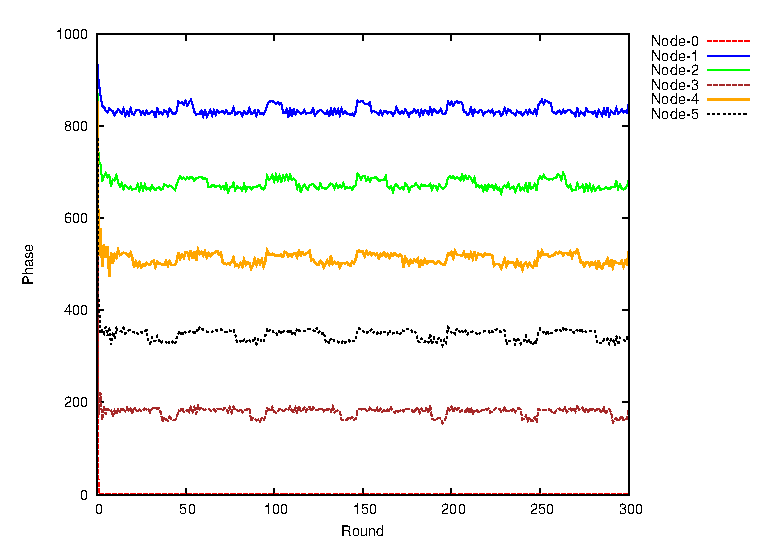
\includegraphics[scale=0.35]{figure/6nodes-star-result-extdesync-good}%
	\label{fig:6nodes-star-result-extdesync-good}}
	\hfil
	\subfloat[LIGHTWEIGHT]{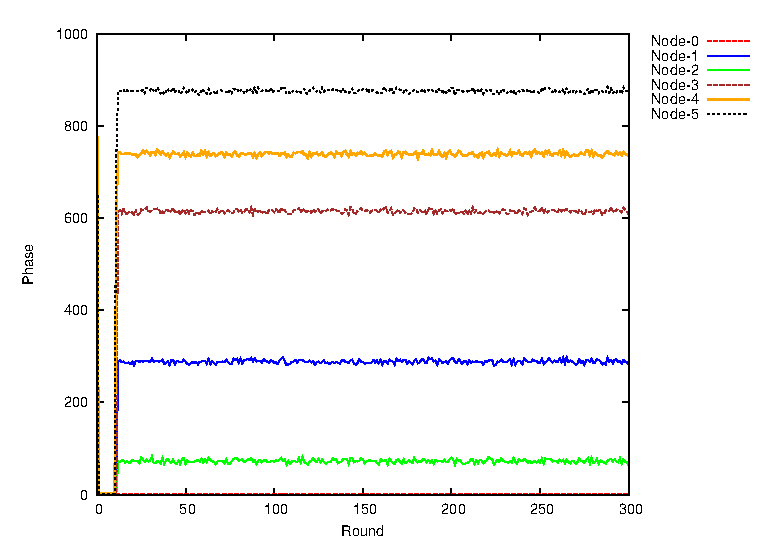
\includegraphics[scale=0.35]{figure/6nodes-star-result-light-good}%
	\label{fig:6nodes-star-result-light-good}}
}
\caption{6-node star topology evaluation (average case).}
\label{fig:6nodes-star-result-good}
\lofcont
\end{figure*}
\begin{figure*}[!t]
\centering{
	\subfloat[M-DWARF]{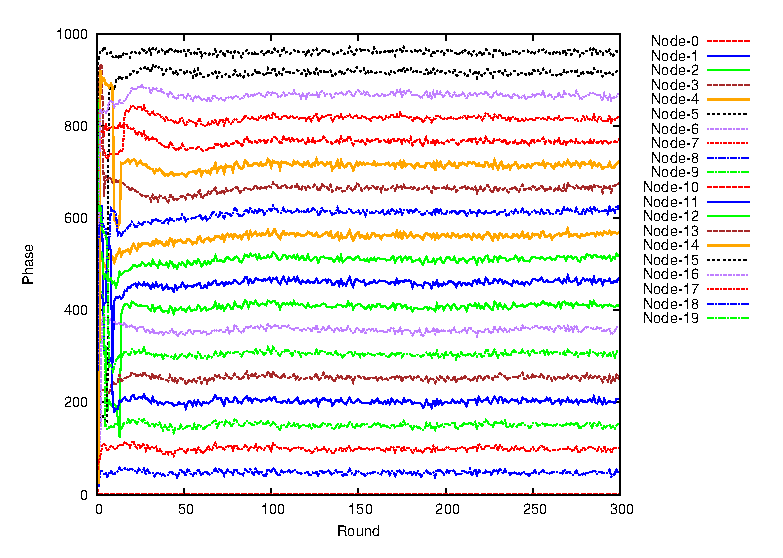
\includegraphics[scale=0.35]{figure/20nodes-star-result-mdwarf-good}%
	\label{fig:20nodes-star-result-mdwarf-good}}
	\hfil
	\subfloat[EXTENDED-DESYNC]{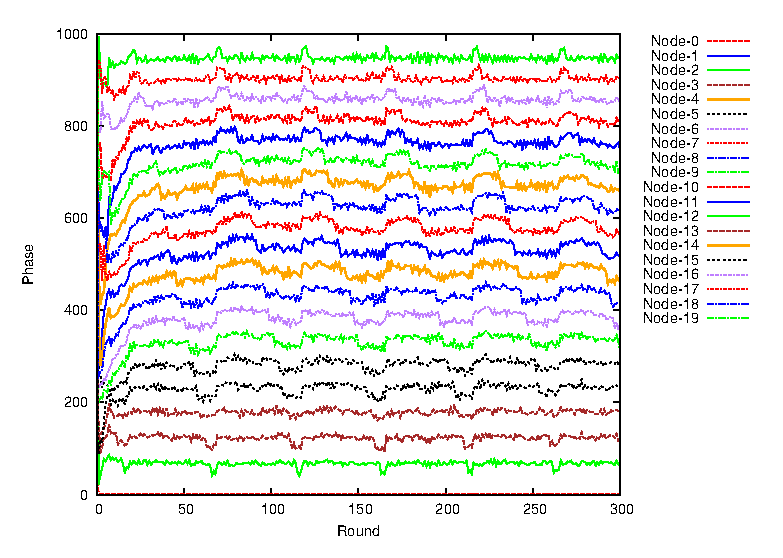
\includegraphics[scale=0.35]{figure/20nodes-star-result-extdesync-good}%
	\label{fig:20nodes-star-result-extdesync-good}}
	\hfil
	\subfloat[LIGHTWEIGHT]{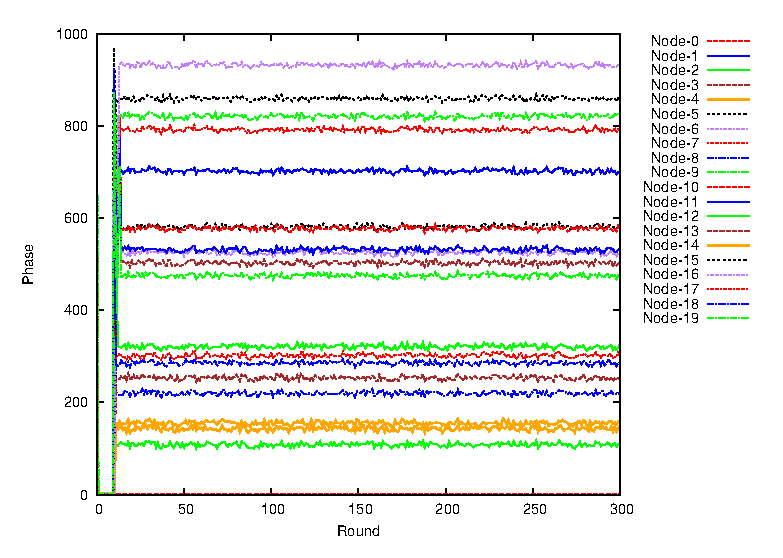
\includegraphics[scale=0.35]{figure/20nodes-star-result-light-good}%
	\label{fig:20nodes-star-result-light-good}}
}
\caption{20-node star topology evaluation (average case).}
\label{fig:20nodes-star-result-good}
\lofcont
\end{figure*}
The star topology is the simplest case for multi-hop desynchronization. There is one center node that can transmit and receive messages with all other nodes in the network. In contrast, other nodes can  transmit and receive only with the center node. Figure \ref{fig:star-eval} illustrates 6-node and 20-node star topologies that we use for algorithms evaluation. In the star topology, every node is connected to each other within two-hop communication. As a result, all nodes must use different time slots. 

Figure \ref{fig:6nodes-star-result-good} and \ref{fig:20nodes-star-result-good} shows the simulation results of three algorithms on 6-node and 20-node star topologies respectively.
Due to the relative phase relaying mechanism, both M-DWARF and EXTENDED-DESYNC perceive relative phases of neighbors within two hops, which are all nodes in the system. Consequently, both algorithms can separate 6 nodes into almost equivalent 6 time slots. However, M-DWARF achieves almost perfect desynchony whereas EXTENDED-DESYNC slightly fluctuates in the sparse 6-node network and highly fluctuates in the dense 20-node network.
\begin{figure*}[!t]
\centering{
	\subfloat[M-DWARF]{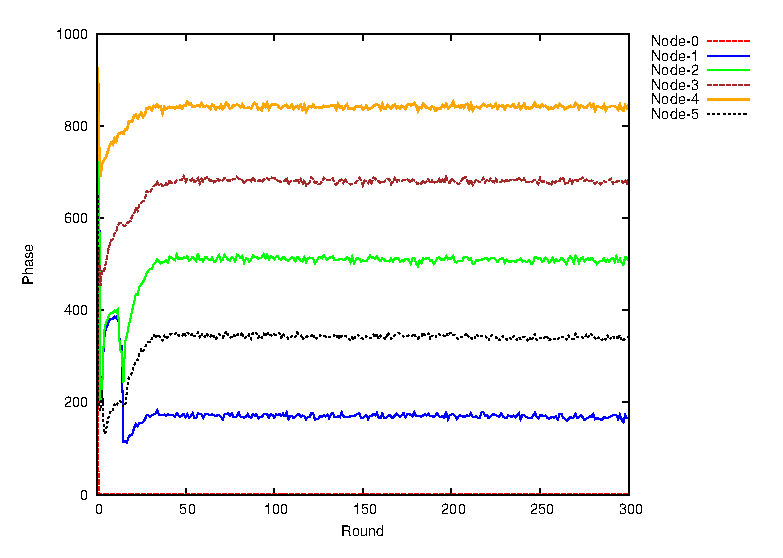
\includegraphics[scale=0.35]{figure/6nodes-star-result-mdwarf-bad}%
	\label{fig:6nodes-star-result-mdwarf-bad}}
	\hfil
	\subfloat[EXTENDED-DESYNC]{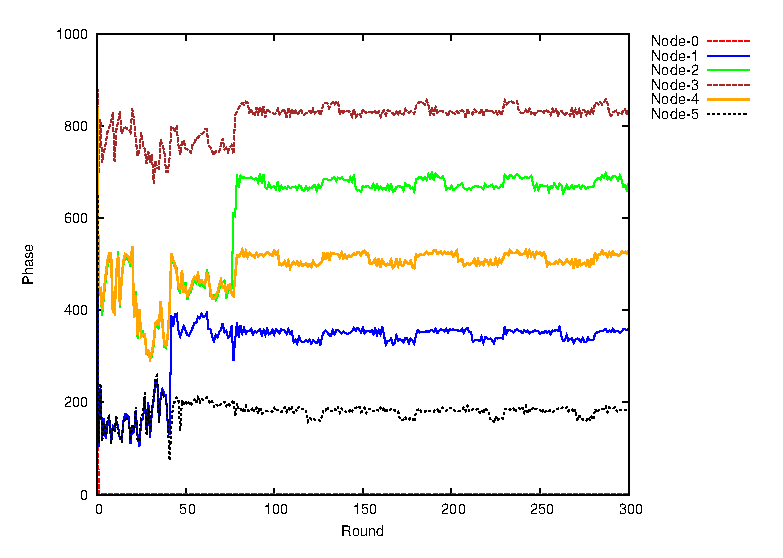
\includegraphics[scale=0.35]{figure/6nodes-star-result-extdesync-bad}%
	\label{fig:6nodes-star-result-extdesync-bad}}
	\hfil
	\subfloat[LIGHTWEIGHT]{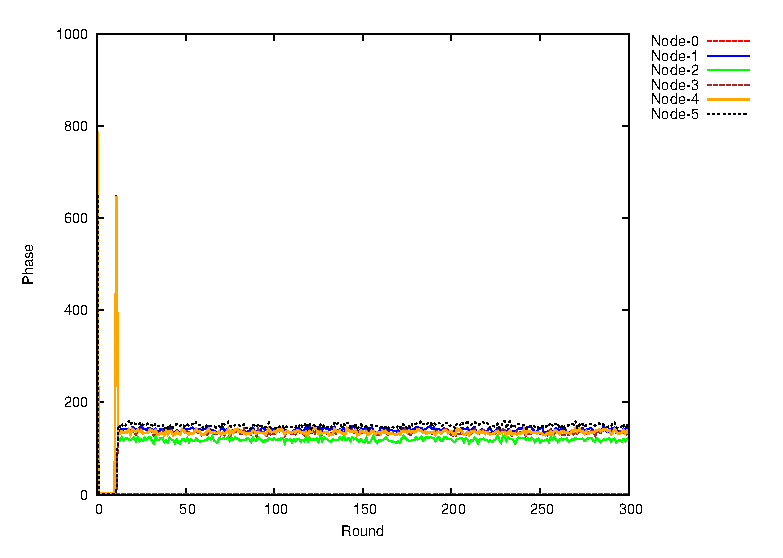
\includegraphics[scale=0.35]{figure/6nodes-star-result-light-bad}%
	\label{fig:6nodes-star-result-light-bad}}
}
\caption{6-node star topology evaluation (problematic case).}
\label{fig:6nodes-star-result-bad}
\lofcont
\end{figure*}
\begin{figure*}[!t]
\centering{
	\subfloat[M-DWARF]{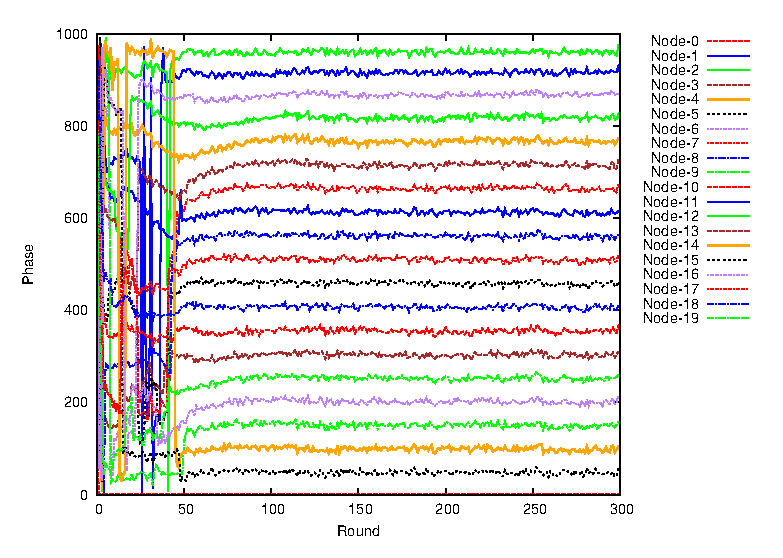
\includegraphics[scale=0.35]{figure/20nodes-star-result-mdwarf-bad}%
	\label{fig:20nodes-star-result-mdwarf-bad}}
	\hfil
	\subfloat[EXTENDED-DESYNC]{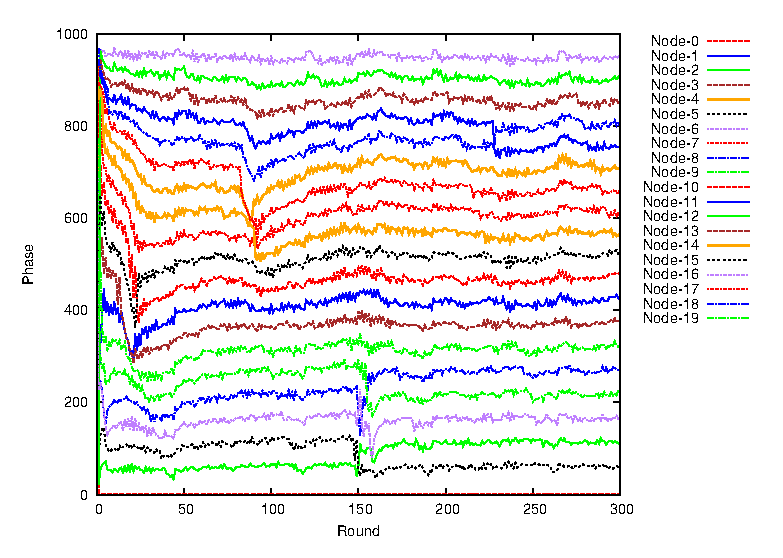
\includegraphics[scale=0.35]{figure/20nodes-star-result-extdesync-bad}%
	\label{fig:20nodes-star-result-extdesync-bad}}
	\hfil
	\subfloat[LIGHTWEIGHT]{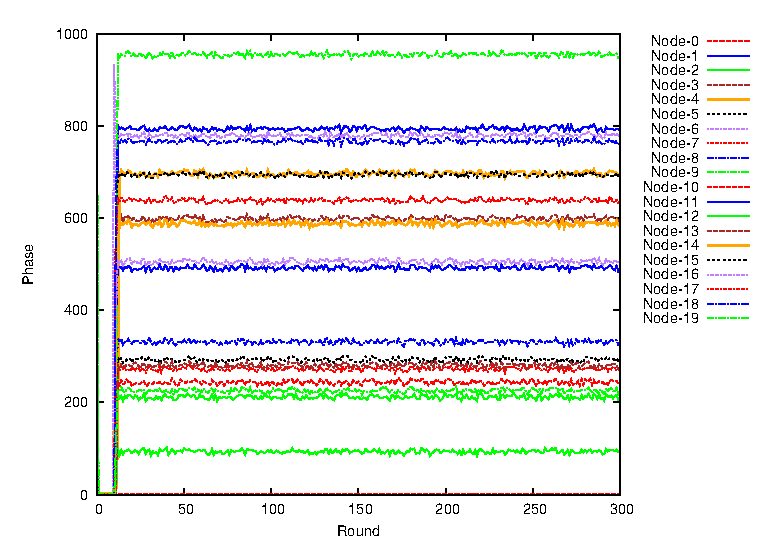
\includegraphics[scale=0.35]{figure/20nodes-star-result-light-bad}%
	\label{fig:20nodes-star-result-light-bad}}
}
\caption{20-node star topology evaluation (problematic case).}
\label{fig:20nodes-star-result-bad}
\lofcont
\end{figure*}
Figure \ref{fig:6nodes-star-result-bad} and \ref{fig:20nodes-star-result-bad} shows the problematic cases. For M-DWARF, there is no problem in the sparse networks, but, in the dense networks, nodes take more time to become stable. The reason is that, when the network is dense, the usable time interval gap for each node is shortened. Therefore, if several nodes start closely to each other at the initial configuration, forces are highly absorbed. As a result, they takes more time to separate away from each other. In the case of EXTENDED-DESYNC, the fluctuated error from one node can propagate throughout the networks because each node relies on only information of two phase neighbors.




\subsubsection{Chain Topology}
The chain topology is one of the simplest topologies. Every node is lined up without a loop. The 3-node and 10-node chain topologies are depicted in Figure \ref{fig:chain-eval}. 
\begin{figure*}[!t]
\centering{
	\subfloat[3 nodes]{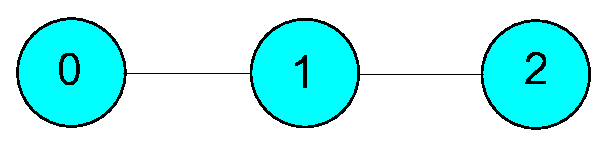
\includegraphics[scale=0.45]{figure/3nodes-chain-eval}%
	\label{fig:3nodes-chain-eval}}
	\hspace{1in}
	\subfloat[10 nodes]{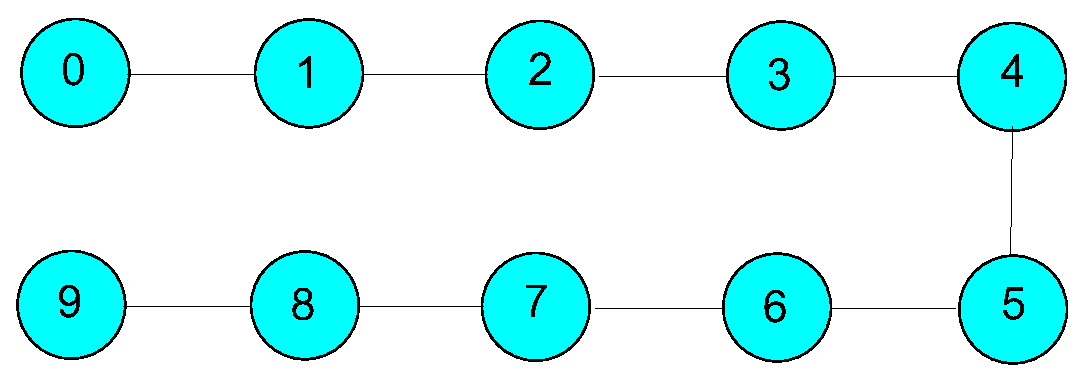
\includegraphics[scale=0.35]{figure/10nodes-chain-eval}%
	\label{fig:10nodes-chain-eval}}
}
\caption{Chain topology}
\label{fig:chain-eval}
\lofcont
\end{figure*}
\begin{figure*}[!t]
\centering{
	\subfloat[M-DWARF]{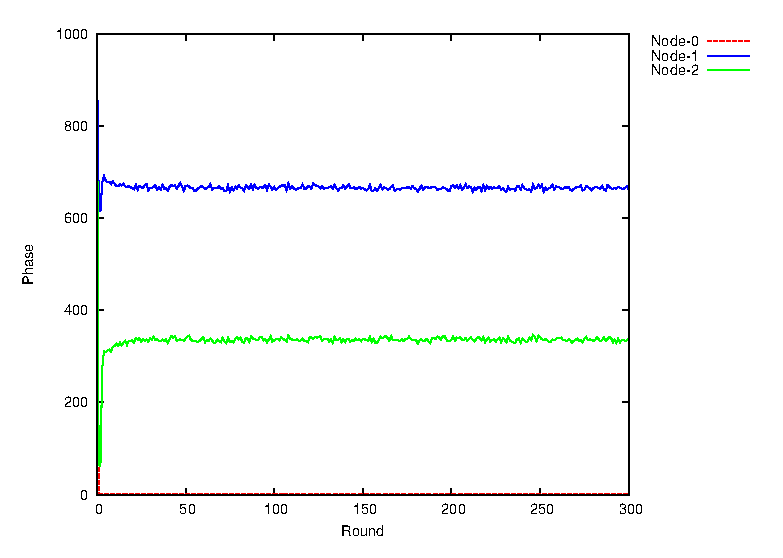
\includegraphics[scale=0.35]{figure/3nodes-chain-result-mdwarf-good}%
	\label{fig:3nodes-chain-result-mdwarf-good}}
	\hfil
	\subfloat[EXTENDED-DESYNC]{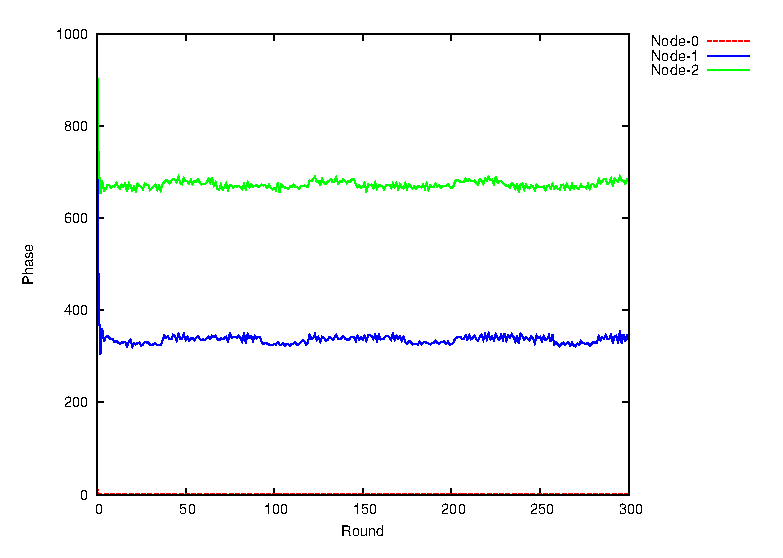
\includegraphics[scale=0.35]{figure/3nodes-chain-result-extdesync-good}%
	\label{fig:3nodes-chain-result-extdesync-good}}
	\hfil
	\subfloat[LIGHTWEIGHT]{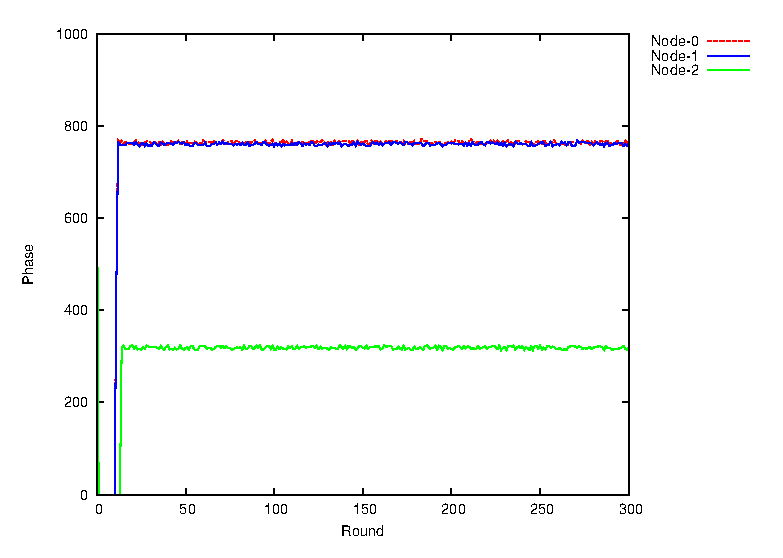
\includegraphics[scale=0.35]{figure/3nodes-chain-result-light-good}%
	\label{fig:3nodes-chain-result-light-good}}
}
\caption{3-node chain topology evaluation (average case).}
\label{fig:3nodes-chain-result-good}
\lofcont
\end{figure*}
\begin{figure*}[!t]
\centering{
	\subfloat[M-DWARF]{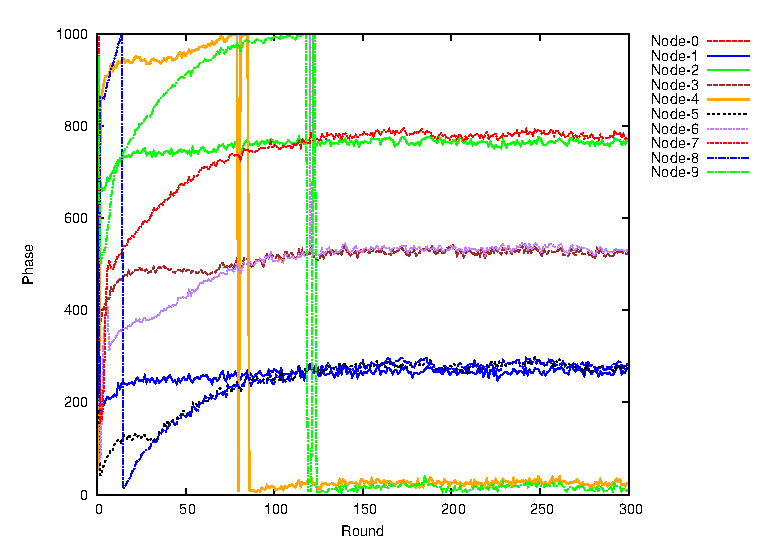
\includegraphics[scale=0.35]{figure/10nodes-chain-result-mdwarf-good}%
	\label{fig:10nodes-chain-result-mdwarf-good}}
	\hfil
	\subfloat[EXTENDED-DESYNC]{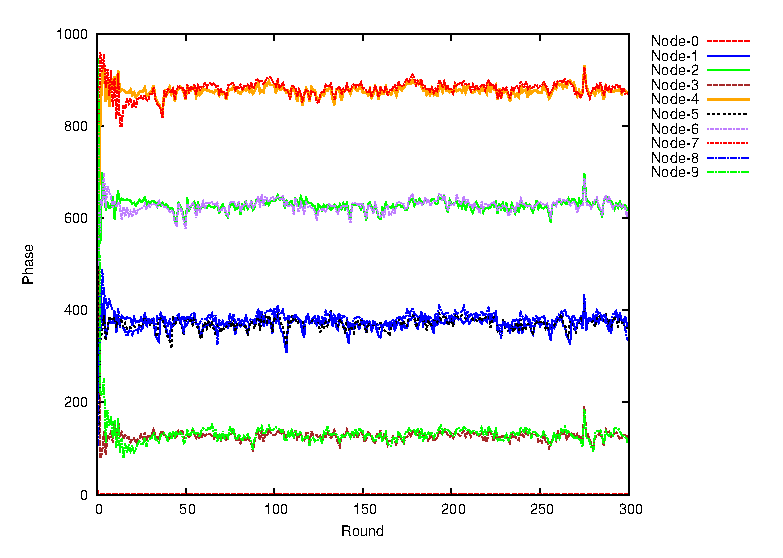
\includegraphics[scale=0.35]{figure/10nodes-chain-result-extdesync-good}%
	\label{fig:10nodes-chain-result-extdesync-good}}
	\hfil
	\subfloat[LIGHTWEIGHT]{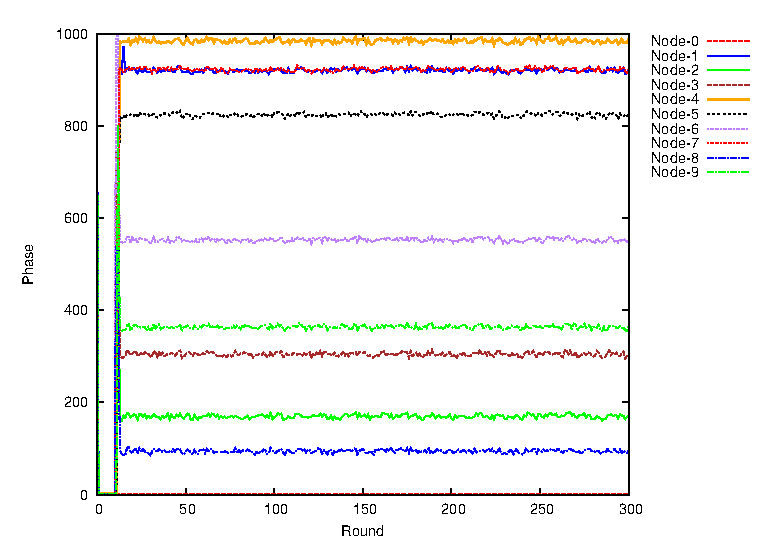
\includegraphics[scale=0.35]{figure/10nodes-chain-result-light-good}%
	\label{fig:10nodes-chain-result-light-good}}
}
\caption{10-node chain topology evaluation (average case).}
\label{fig:10nodes-chain-result-good}
\lofcont
\end{figure*}
For 3 nodes, this case is simple because all three nodes cannot share  the same phase.
In most cases as shown in Figure \ref{fig:3nodes-chain-result-good}, both M-DWARF and EXTENDED-DESYNC perform very well. All nodes are equivalently separated. However, M-DWARF is slightly smoother than EXTENDED-DESYNC. 

For 10 nodes, some nodes that are farther than two hops are able to use the same phase. There are several optimal solutions. For exmaple, the first optimal solution is that there are four groups of nodes that use different phases. Each node within the same group can use the same phase. These four groups are $\lbrace 0, 3, 6, 9 \rbrace , \lbrace 1, 4, 7 \rbrace, \lbrace 2, 5, 8 \rbrace$, and $\lbrace 6 \rbrace$. Another optimal solution is $\lbrace 0, 4, 9 \rbrace, \lbrace 1, 5, 8 \rbrace, \lbrace 3, 6 \rbrace,$ and $\lbrace 2, 7 \rbrace$.
We note that, in our 30 simulations, M-DWARF could achieve the perfect desynchrony state with 4 slots as in Figure \ref{fig:10nodes-chain-result-mdwarf-good}, but EXTENDED-DEESYNC never achieve the perfect desynchrony state (there are 5 slots in Figure \ref{fig:10nodes-chain-result-extdesync-good} because node 0 is at phase 0).

\begin{figure*}[!t]
\centering{
	\subfloat[M-DWARF]{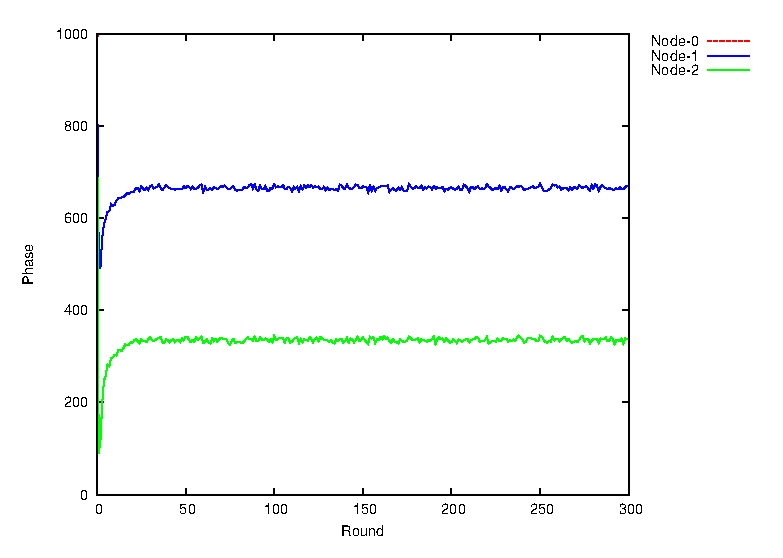
\includegraphics[scale=0.35]{figure/3nodes-chain-result-mdwarf-bad}%
	\label{fig:3nodes-chain-result-mdwarf-bad}}
	\hfil
	\subfloat[EXTENDED-DESYNC]{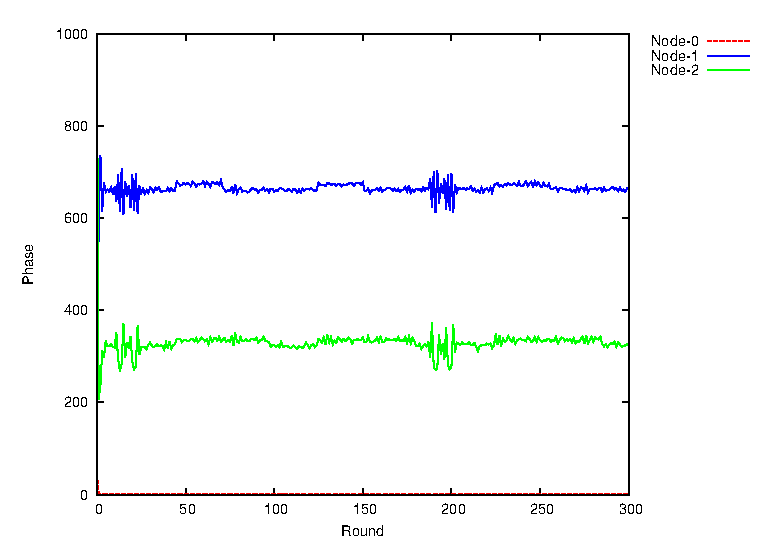
\includegraphics[scale=0.35]{figure/3nodes-chain-result-extdesync-bad}%
	\label{fig:3nodes-chain-result-extdesync-bad}}
	\hfil
	\subfloat[LIGHTWEIGHT]{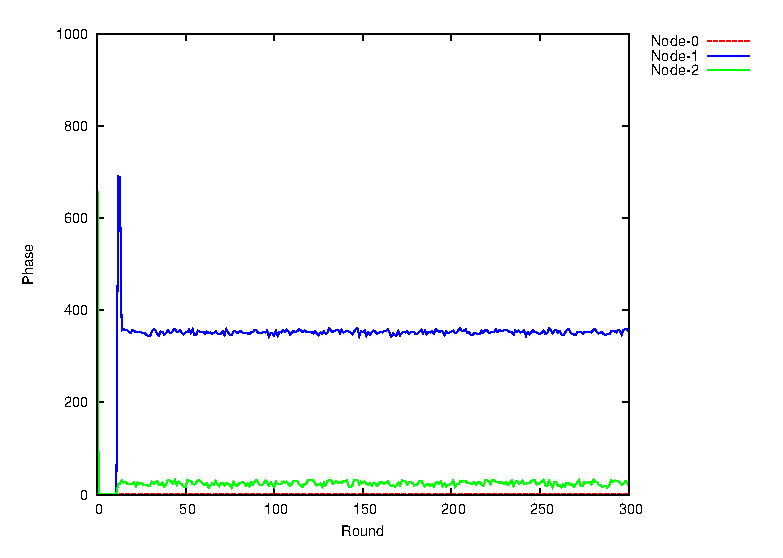
\includegraphics[scale=0.35]{figure/3nodes-chain-result-light-bad}%
	\label{fig:3nodes-chain-result-light-bad}}
}
\caption{3-node chain topology evaluation (problematic case).}
\label{fig:3nodes-chain-result-bad}
\lofcont
\end{figure*}
\begin{figure*}[!t]
\centering{
	\subfloat[M-DWARF]{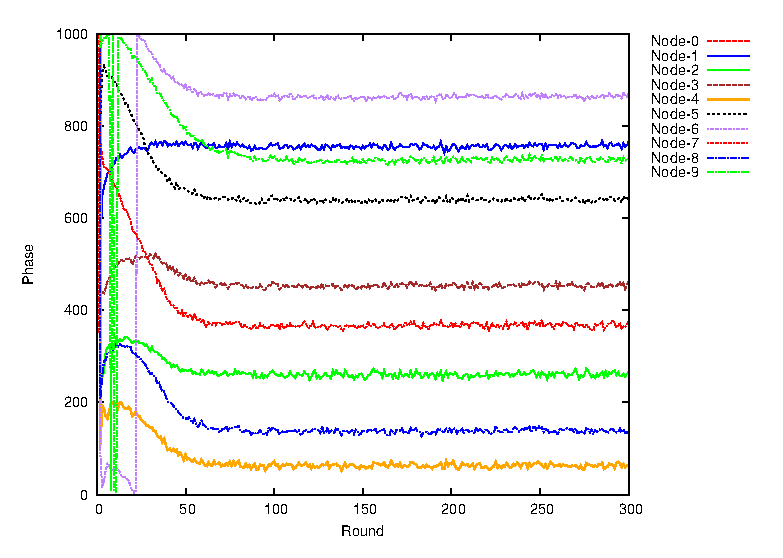
\includegraphics[scale=0.35]{figure/10nodes-chain-result-mdwarf-bad}%
	\label{fig:10nodes-chain-result-mdwarf-bad}}
	\hfil
	\subfloat[EXTENDED-DESYNC]{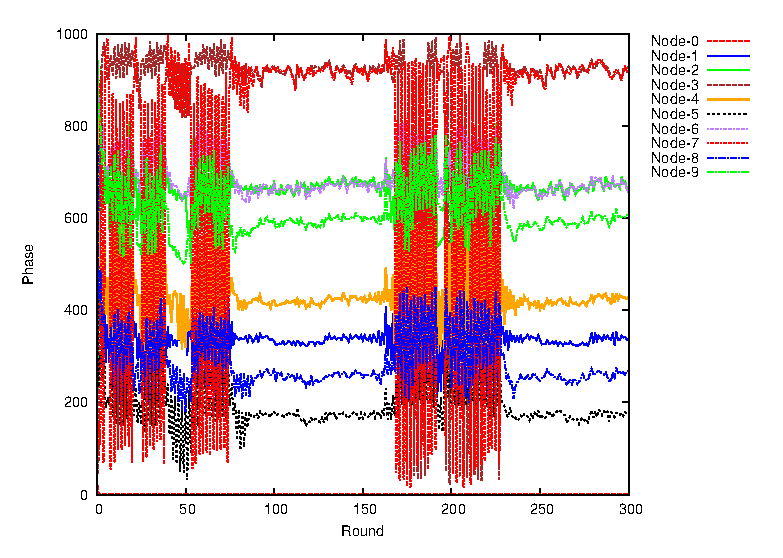
\includegraphics[scale=0.35]{figure/10nodes-chain-result-extdesync-bad}%
	\label{fig:10nodes-chain-result-extdesync-bad}}
	\hfil
	\subfloat[LIGHTWEIGHT]{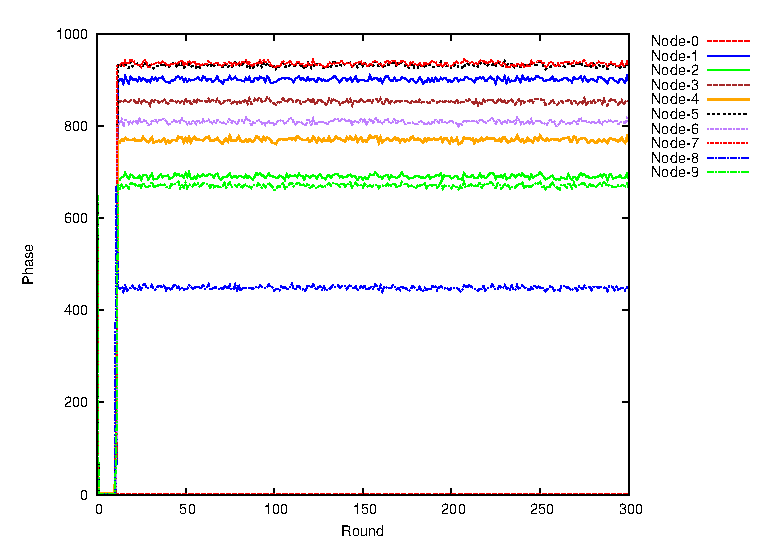
\includegraphics[scale=0.35]{figure/10nodes-chain-result-light-bad}%
	\label{fig:10nodes-chain-result-light-bad}}
}
\caption{10-node chain topology evaluation (problematic case).}
\label{fig:10nodes-chain-result-bad}
\lofcont
\end{figure*}
In some problematic cases, the phases of EXTENDED-DESYNC are slightly fluctuate in the sparse networks (Figure \ref{fig:3nodes-chain-result-extdesync-bad}) and highly fluctuate in the dense networks (Figure \ref{fig:10nodes-chain-result-extdesync-bad}). Additionally, for both EXTENDED-DESYNC and M-DWARF, each node attempts to gradually adjust its phase in the range between previous and next phase neighbors. Therefore, if the initial configuration is not proper, nodes may be not able to adjust their phases over the range of such neighbors and the networks cannot get into the perfect desynchrony state. Figure \ref{fig:10nodes-chain-result-mdwarf-bad} and \ref{fig:10nodes-chain-result-extdesync-bad} illustrate this problem.

\subsubsection{Cycle Topology}
The cycle topology is simlar to the chain topology. All nodes are lined up but the first and last nodes are connected together to form a closed loop. Figure \ref{fig:cycle-eval} depicts 4-node and 10-node cycle topologies.
\begin{figure*}[!t]
\centering{
	\subfloat[4 nodes]{\includegraphics[scale=0.4]{figure/4nodes-cycle-eval}%
	\label{fig:4nodes-cycle-eval}}
	\hspace{1in}
	\subfloat[10 nodes]{\includegraphics[scale=0.35]{figure/10nodes-cycle-eval}%
	\label{fig:10nodes-cycle-eval}}
}
\caption{Cycle topology}
\label{fig:cycle-eval}
\lofcont
\end{figure*}

\begin{figure*}[!t]
\centering{
	\subfloat[M-DWARF]{\includegraphics[scale=0.35]{figure/4nodes-cycle-result-mdwarf-good}%
	\label{fig:4nodes-cycle-result-mdwarf-good}}
	\hfil
	\subfloat[EXTENDED-DESYNC]{\includegraphics[scale=0.35]{figure/4nodes-cycle-result-extdesync-good}%
	\label{fig:4nodes-cycle-result-extdesync-good}}
	\hfil
	\subfloat[LIGHTWEIGHT]{\includegraphics[scale=0.35]{figure/4nodes-cycle-result-light-good}%
	\label{fig:4nodes-cycle-result-light-good}}
}
\caption{4-node cycle topology evaluation (average case).}
\label{fig:4nodes-cycle-result-good}
\lofcont
\end{figure*}

\begin{figure*}[!t]
\centering{
	\subfloat[M-DWARF]{\includegraphics[scale=0.35]{figure/10nodes-cycle-result-mdwarf-good}%
	\label{fig:10nodes-cycle-result-mdwarf-good}}
	\hfil
	\subfloat[EXTENDED-DESYNC]{\includegraphics[scale=0.35]{figure/10nodes-cycle-result-extdesync-good}%
	\label{fig:10nodes-cycle-result-extdesync-good}}
	\hfil
	\subfloat[LIGHTWEIGHT]{\includegraphics[scale=0.35]{figure/10nodes-cycle-result-light-good}%
	\label{fig:10nodes-cycle-result-light-good}}
}
\caption{10-node cycle topology evaluation (average case).}
\label{fig:10nodes-cycle-result-good}
\lofcont
\end{figure*}
For 4-node cycle networks, all nodes are within two hops from each other. Therefore, every node knows phases of other nodes and no node shares the same phase. On average, both M-DWARF and EXTENDED-DESYNC achieve the perfect desynchrony state as shown in Figure \ref{fig:4nodes-cycle-result-mdwarf-good} and \ref{fig:4nodes-cycle-result-extdesync-good}. For 10-node networks, some optimal solutions are different from the optimal solutions in the case of the 10-node chain topology because node 0 and 9 cannot share the same phase in the cycle topology. Both M-DWARF and EXTENDED-DESYNCE can achieve the perfect desynchrony state in this case (see Figure \ref{fig:10nodes-cycle-result-mdwarf-good} and \ref{fig:10nodes-cycle-result-extdesync-good}). However, again, the phases of EXTENDED-DESYNC are fluctuate.

In some problematic cases, the result is similar to the problematic result of the chain topology with the same reason that the initial configuration affects how nodes adjust theirs phases to the proper phases. Figure \ref{fig:4nodes-cycle-result-mdwarf-bad}, \ref{fig:4nodes-cycle-result-extdesync-bad}, \ref{fig:10nodes-cycle-result-mdwarf-bad}, and \ref{fig:10nodes-cycle-result-extdesync-bad} illustrate the problem.

\begin{figure*}[!t]
\centering{
	\subfloat[M-DWARF]{\includegraphics[scale=0.35]{figure/4nodes-cycle-result-mdwarf-bad}%
	\label{fig:4nodes-cycle-result-mdwarf-bad}}
	\hfil
	\subfloat[EXTENDED-DESYNC]{\includegraphics[scale=0.35]{figure/4nodes-cycle-result-extdesync-bad}%
	\label{fig:4nodes-cycle-result-extdesync-bad}}
	\hfil
	\subfloat[LIGHTWEIGHT]{\includegraphics[scale=0.35]{figure/4nodes-cycle-result-light-bad}%
	\label{fig:4nodes-cycle-result-light-bad}}
}
\caption{4-node cycle topology evaluation (problematic case).}
\label{fig:4nodes-cycle-result-bad}
\lofcont
\end{figure*}


\begin{figure*}[!t]
\centering{
	\subfloat[M-DWARF]{\includegraphics[scale=0.35]{figure/10nodes-cycle-result-mdwarf-bad}%
	\label{fig:10nodes-cycle-result-mdwarf-bad}}
	\hfil
	\subfloat[EXTENDED-DESYNC]{\includegraphics[scale=0.35]{figure/10nodes-cycle-result-extdesync-bad}%
	\label{fig:10nodes-cycle-result-extdesync-bad}}
	\hfil
	\subfloat[LIGHTWEIGHT]{\includegraphics[scale=0.35]{figure/10nodes-cycle-result-light-bad}%
	\label{fig:10nodes-cycle-result-light-bad}}
}
\caption{10-node cycle topology evaluation (problematic case).}
\label{fig:10nodes-cycle-result-bad}
\lofcont
\end{figure*}

\begin{figure*}[!t]
\centering{
	\subfloat[6 nodes]{\includegraphics[scale=0.3]{figure/6nodes-butterfly-eval}%
	\label{fig:6nodes-butterfly-eval}}
	\hspace{1in}
	\subfloat[20 nodes]{\includegraphics[scale=0.3]{figure/20nodes-butterfly-eval}%
	\label{fig:20nodes-butterfly-eval}}
}
\caption{Dumbbell topology}
\label{fig:butterfly-eval}
\lofcont
\end{figure*}

\subsubsection{Dumbbell Topology}
\begin{figure*}[!t]
\centerline{
	\subfloat[M-DWARF]{\includegraphics[scale=0.35]{figure/6nodes-butterfly-result-mdwarf-good}%
	\label{fig:6nodes-butterfly-result-mdwarf-good}}
	\hfil
	\subfloat[EXTENDED-DESYNC]{\includegraphics[scale=0.35]{figure/6nodes-butterfly-result-extdesync-good}%
	\label{fig:6nodes-butterfly-result-extdesync-good}}
	\hfil
	\subfloat[LIGHTWEIGHT]{\includegraphics[scale=0.35]{figure/6nodes-butterfly-result-light-good}%
	\label{fig:6nodes-butterfly-result-light-good}}
}
\caption{6-node dumbbell topology evaluation (average case).}
\label{fig:6nodes-butterfly-result-good}
\lofcont
\end{figure*}

\begin{figure*}[!t]
\centerline{
	\subfloat[M-DWARF]{\includegraphics[scale=0.35]{figure/20nodes-butterfly-result-mdwarf-good}%
	\label{fig:20nodes-butterfly-result-mdwarf-good}}
	\hfil
	\subfloat[EXTENDED-DESYNC]{\includegraphics[scale=0.35]{figure/20nodes-butterfly-result-extdesync-good}%
	\label{fig:20nodes-butterfly-result-extdesync-good}}
	\hfil
	\subfloat[LIGHTWEIGHT]{\includegraphics[scale=0.35]{figure/20nodes-butterfly-result-light-good}%
	\label{fig:20nodes-butterfly-result-light-good}}
}
\caption{20-node dumbbell topology evaluation (average case).}
\label{fig:20nodes-butterfly-result-good}
\lofcont
\end{figure*}
The dumbbell topology is commonly used in practice. It is one form of the transit-stub networks. In a dumbbell network, there are a number of nodes connected to a single relay node. The relay node is connected to another relay node at another side. Another number of nodes are connected to that final relay node to create a dumbbell topology. Figure \ref{fig:butterfly-eval} depicts 6-node and 20-node dumbbell networks.

Obviously, a node at one end can share the same phase with another node at the other end because they are far from each other beyond two hops. Therefore, for 6-node networks, the optimal solution requires 4 slots. Each slot interval is $T/4$. For 20-node networks, the optimal solution requires 11 slots. Each slot interval is $T/11$.
In Figure \ref{fig:6nodes-butterfly-result-mdwarf-good} and \ref{fig:6nodes-butterfly-result-extdesync-good}, both M-DWARF and EXTENDED-DESYNC achieve the optimal solution for 6-node networks. However, again, M-DWARF is more stable than EXTENDED-DESYNC.

When the network is dense, EXTENDED-DESYNC is highly fluctuate. If one node adapts their phase too fast, several nodes are affected because there are many two-hop neighbors in the dumbbell networks as illustrated in Figure \ref{fig:20nodes-butterfly-result-extdesync-bad}.  In contrast, in M-DWARF, the fast adaptation of one node does not has high impact to other nodes because nodes do not rely on only their two phase neighbors but use all information from neighbors within two hops as the force function.

\begin{figure*}[!t]
\centerline{
	\subfloat[M-DWARF]{\includegraphics[scale=0.35]{figure/6nodes-butterfly-result-mdwarf-bad}%
	\label{fig:6nodes-butterfly-result-mdwarf-bad}}
	\hfil
	\subfloat[EXTENDED-DESYNC]{\includegraphics[scale=0.35]{figure/6nodes-butterfly-result-extdesync-bad}%
	\label{fig:6nodes-butterfly-result-extdesync-bad}}
	\hfil
	\subfloat[LIGHTWEIGHT]{\includegraphics[scale=0.35]{figure/6nodes-butterfly-result-light-bad}%
	\label{fig:6nodes-butterfly-result-light-bad}}
}
\caption{6-node dumbbell topology evaluation (problematic case).}
\label{fig:6nodes-butterfly-result-bad}
\lofcont
\end{figure*}

\begin{figure*}[!t]
\centerline{
	\subfloat[M-DWARF]{\includegraphics[scale=0.35]{figure/20nodes-butterfly-result-mdwarf-bad}%
	\label{fig:20nodes-butterfly-result-mdwarf-bad}}
	\hfil
	\subfloat[EXTENDED-DESYNC]{\includegraphics[scale=0.35]{figure/20nodes-butterfly-result-extdesync-bad}%
	\label{fig:20nodes-butterfly-result-extdesync-bad}}
	\hfil
	\subfloat[LIGHTWEIGHT]{\includegraphics[scale=0.35]{figure/20nodes-butterfly-result-light-bad}%
	\label{fig:20nodes-butterfly-result-light-bad}}
}
\caption{20-node dumbbell topology evaluation (problematic case).}
\label{fig:20nodes-butterfly-result-bad}
\lofcont
\end{figure*}

\subsubsection{Mesh Topology}
We use the 10-node mesh topology described in \cite{4663417} as depicted in Figure \ref{fig:10nodes-topo}. A solid line represents one-hop connectivity whereas a dash line represents two-hop connectivity. In \cite{4663417}, they state the best case of this topology is that eight slots are required. However, in our simulation, we discover the better solution that requires only six slots as illustrated in Figure \ref{fig:10nodes-mesh-result-mdwarf-good} for M-DWARF and Figure \ref{fig:10nodes-mesh-result-extdesync-good} for EXTENDED-DESYNC. The problematic case for bot M-DWARF and EXTENDED-DESYNC is that the initial configuration is not proper. However, as expected, EXTENDED-DESYNCE is affected from highly fluctuation.
\begin{figure}[!t]
\centering
\includegraphics[width=3in]{figure/10nodes-topo-mhop}
\caption{10-node multi-hop network. A solid line represents 1-hop connectivity. A dash line represents 2-hop connectivity. Any two nodes that are connected within 2-hop connectivity can interfere each other transmission.}
\label{fig:10nodes-topo}
\end{figure}

\begin{figure*}[!t]
\centerline{
	\subfloat[M-DWARF]{\includegraphics[scale=0.35]{figure/10nodes-mesh-result-mdwarf-good}%
	\label{fig:10nodes-mesh-result-mdwarf-good}}
	\hfil
	\subfloat[EXTENDED-DESYNC]{\includegraphics[scale=0.35]{figure/10nodes-mesh-result-extdesync-good}%
	\label{fig:10nodes-mesh-result-extdesync-good}}
	\hfil
	\subfloat[LIGHTWEIGHT]{\includegraphics[scale=0.35]{figure/10nodes-mesh-result-light-good}%
	\label{fig:10nodes-mesh-result-light-good}}
}
\caption{10-node mesh topology evaluation (average case).}
\label{fig:10nodes-mesh-result-good}
\lofcont
\end{figure*}
\begin{figure*}[!t]
\centerline{
	\subfloat[M-DWARF]{\includegraphics[scale=0.35]{figure/10nodes-mesh-result-mdwarf-bad}%
	\label{fig:10nodes-mesh-result-mdwarf-bad}}
	\hfil
	\subfloat[EXTENDED-DESYNC]{\includegraphics[scale=0.35]{figure/10nodes-mesh-result-extdesync-bad}%
	\label{fig:10nodes-mesh-result-extdesync-bad}}
	\hfil
	\subfloat[LIGHTWEIGHT]{\includegraphics[scale=0.35]{figure/10nodes-mesh-result-light-bad}%
	\label{fig:10nodes-mesh-result-light-bad}}
}
\caption{10-node mesh topology evaluation (problematic case).}
\label{fig:10nodes-mesh-result-bad}
\lofcont
\end{figure*}

\subsection{Impact of Period Length}
In previous experiments, we set the time period to 1,000 milliseconds. In this experiment, we vary the period from 1,000 to 3,000 milliseconds. To obviously see the impact of period length, we use the star topology which is the multi-hop topology that all nodes perceive all 2-hop neighbors and set the number of nodes to 30 nodes.
With this topology and the number of nodes, the network is saturated within the 1,000-millisecond period. 

Figure \ref{fig:period-mdwarf} and \ref{fig:period-ext} show the phase graphs when varying period length of M-DWARF and EXTENDED-DESYNC respectively. At the 1,000-millisecond period, the network is saturated for 30 nodes. 
First, we notice that this result is different from 30 nodes in the single-hop networks that we evaluate in Chapter \ref{chap:algo} which nodes are well-spread in a time period. 
In the single-hop DWARF algorithm, a firing message does not contain any overhead, whereas, in the multi-hop M-DWARF algorithm, a firing message contains one-hop neighbors relative phases.
Therefore, the firing message of multi-hop M-DWARF takes longer firing time than that of single-hop DWARF.
Consequently, the time gap between two firing messages is reduced in M-DWARF.

With the same period length, there are more nodes in EXTENDED-DESYNC than in M-DWARF that stay at the same phase and their firing messages collide. When the period length is increased to 2,000 and 3,000 milliseconds, the free time gap is also increased. Therefore, the number of collisions is reduced and nodes are better spread in both algorithms. 


\begin{figure*}[!t]
\centerline{
	\subfloat[$T$ = 1000 ms]{\includegraphics[scale=0.35]{figure/period1000-mdwarf}%
	\label{fig:period1000-mdwarf}}
	\hfil
	\subfloat[$T$ = 2000 ms]{\includegraphics[scale=0.35]{figure/period2000-mdwarf}%
	\label{fig:period2000-mdwarf}}
	\hfil
	\subfloat[$T$ = 3000 ms]{\includegraphics[scale=0.35]{figure/period3000-mdwarf}%
	\label{fig:period3000-mdwarf}}
}
\caption{Impact of period length ($T$) in M-DWARF}
\label{fig:period-mdwarf}
\lofcont
\end{figure*}
\begin{figure*}[!t]
\centerline{
	\subfloat[$T$ = 1000 ms]{\includegraphics[scale=0.35]{figure/period1000-ext}%
	\label{fig:period1000-ext}}
	\hfil
	\subfloat[$T$ = 2000 ms]{\includegraphics[scale=0.35]{figure/period2000-ext}%
	\label{fig:period2000-ext}}
	\hfil
	\subfloat[$T$ = 3000 ms]{\includegraphics[scale=0.35]{figure/period3000-ext}%
	\label{fig:period3000-ext}}
}
\caption{Impact of period length ($T$) in EXTENDED-DESYNC}
\label{fig:period-ext}
\lofcont
\end{figure*}

\subsection{Channel Utilization and Fairness}
In this section, we measure the average channel utilization of M-DWARF and EXTENDED-DESYNC. The channel can be utilized by one node if there is no collision during an amount of time between a node's firing to another node's firing. 
Figure \ref{fig:period-overallthroughput-30-40} shows the results of networks with 30 and 40 nodes and Figure \ref{fig:period-overallthroughput-50-60} shows the results of networks with 50 and 60 nodes.
At the 1000-millisecond period, the average channel utilizations of 30 to 60 nodes networks are almost the same because the network are already saturated and there are several collisions. The number of colliding nodes are also approximately the same for both algorithms.
When the period length is increased, M-DWARF performs better than EXTENDED-DESYNC because there are less collisions in M-DWARF. However, we note that this benefit is not significant (only around 50 milliseconds improvement).


\begin{figure*}[!t]
\centerline{
	\subfloat[$T$ = 1000 ms]{\includegraphics[scale=0.65]{figure/period1000-compare-overallthroughput-30-40nodes-sd}%
	\label{fig:period1000-overallthroughput-30-40}}
	\hfil
	\subfloat[$T$ = 2000 ms]{\includegraphics[scale=0.65]{figure/period2000-compare-overallthroughput-30-40nodes-sd}%
	\label{fig:period2000-overallthroughput-30-40}}
	\hfil
	\subfloat[$T$ = 3000 ms]{\includegraphics[scale=0.65]{figure/period3000-compare-overallthroughput-30-40nodes-sd}%
	\label{fig:period3000-overallthroughput-30-40}}
}
\caption{Average channel utilization of 30 and 40 node networks}
\label{fig:period-overallthroughput-30-40}
\lofcont
\end{figure*}

\begin{figure*}[!t]
\centerline{
	\subfloat[$T$ = 1000 ms]{\includegraphics[scale=0.65]{figure/period1000-compare-overallthroughput-50-60nodes-sd}%
	\label{fig:period1000-overallthroughput-50-60}}
	\hfil
	\subfloat[$T$ = 2000 ms]{\includegraphics[scale=0.65]{figure/period2000-compare-overallthroughput-50-60nodes-sd}%
	\label{fig:period2000-overallthroughput-50-60}}
	\hfil
	\subfloat[$T$ = 3000 ms]{\includegraphics[scale=0.65]{figure/period3000-compare-overallthroughput-50-60nodes-sd}%
	\label{fig:period3000-overallthroughput-50-60}}
}
\caption{Average channel utilization of 50 and 60 node networks}
\label{fig:period-overallthroughput-50-60}
\lofcont
\end{figure*}

Then, we measure the fairness of nodes utilizing the channel. If we average the channel utilization per node, the result is approximately the same for M-DWARF and EXTENDED-DESYNC but M-DWARF is insignificantly slightly better (which is the reason why the average channel utilization of M-DWARF is only slightly better). However, to measure the fairness, we are interested in the value of the average standard deviation of the channel utilization per node. If nodes fairly utilize the network, this value is low.
The results of 30 and 40 nodes networks are shown in Figure \ref{fig:period-fairness-30-40} and the results of 50 and 60 nodes networks are shown in Figure \ref{fig:period-fairness-50-60}.
In saturated networks (\textit{i.e.} 1000-millisecond period), the fairness of both M-DWARF and EXTENDED-DESYNC is approximately the same when the time passes. However, the difference of fairness becomes significantly large when the period length is increased. The average standard deviation of the channel utilization per node of EXTENDED-DESYNC is 30 - 400\% higher than that of M-DWARF. Therefore, M-DWARF achieves better fairness. One of the main reasons that nodes in M-DWARF fairly utilize a network is that the stability of M-DWARF is better than that of EXTENDED-DESYNC which still has error-fluctuation (see Chapter \ref{chap:algo}).

\begin{figure*}[!t]
\centerline{
	\subfloat[$T$ = 1000 ms]{\includegraphics[scale=0.65]{figure/period1000-compare-sd-throughputpernode-30-40nodes-sd}%
	\label{fig:period1000-fairness-30-40}}
	\hfil
	\subfloat[$T$ = 2000 ms]{\includegraphics[scale=0.65]{figure/period2000-compare-sd-throughputpernode-30-40nodes-sd}%
	\label{fig:period2000-fairness-30-40}}
	\hfil
	\subfloat[$T$ = 3000 ms]{\includegraphics[scale=0.65]{figure/period3000-compare-sd-throughputpernode-30-40nodes-sd}%
	\label{fig:period3000-fairness-30-40}}
}
\caption{Average standard deviation of channel utilization per node of 30 and 40 node networks}
\label{fig:period-fairness-30-40}
\lofcont
\end{figure*}

\begin{figure*}[!t]
\centerline{
	\subfloat[$T$ = 1000 ms]{\includegraphics[scale=0.65]{figure/period1000-compare-sd-throughputpernode-50-60nodes-sd}%
	\label{fig:period1000-fairness-50-60}}
	\hfil
	\subfloat[$T$ = 2000 ms]{\includegraphics[scale=0.65]{figure/period2000-compare-sd-throughputpernode-50-60nodes-sd}%
	\label{fig:period2000-fairness-50-60}}
	\hfil
	\subfloat[$T$ = 3000 ms]{\includegraphics[scale=0.65]{figure/period3000-compare-sd-throughputpernode-50-60nodes-sd}%
	\label{fig:period3000-fairness-50-60}}
}
\caption{Average standard deviation of channel utilization per node of 50 and 60 node networks}
\label{fig:period-fairness-50-60}
\lofcont
\end{figure*}


\subsection{Overhead Optimization and Robustness to Loss}
Due to the fact that the firing message contains relative phases of one-hop neighbors. If there are too many neighbors, the algorithm incurs large overhead. Therefore, in this evaluation, we attempt to reduce such overhead. We straightforwardly reduce the number of relative phases broadcastings. We only periodically attach neighbors' relative phases in a firing message. Therefore, in most firing messages, relative phases are not included. 
Each node keeps track of phase neighbors within two hops even it does not receive a new firing message. We set a time-to-live for each record to 3 periods. If a node does not receive the phase information from arbitrary node within 3 periods, it removes that node from its records.
To investigate how much we can reduce the overhead, we vary a saving gain parameter $\beta$ which is the frequency to exclude relative phases from a firing message; for example, $\beta  = 0$ means including relative phases in every firing message, $\beta = 1$ means including relative phases in every two firing messages, $\beta = 2$ means including relative phases in every three firing messages, and so on. 

We evaluate this optimization scheme on the 10-node star topology. We vary the saving gain $\beta$ from 0 to 20. 
The result is shown in Figure \ref{fig:vary-saving}.
From the figure, we find that, even we reduce the number of relative phases broadcastings, the system still converges to the perfect desynchrony state in most cases. However, if the saving gain is greater than 16, the system converges slowly or may not converge because the information that a node keeps is removed.
This result indicates two important insights.
First, by trading off with convergence speed, we can drastically reduce the overhead by a factor of 16 in our investigated scenario. Second, even each node does not receive relative phases for many consecutive times. The algorithm still works. Therefore, the proposed algorithm tolerates to packet loss.

\begin{figure*}%
\centering {
	\subfloat[$\beta$ = 0]{\includegraphics[width=2.5in]{figure/beta-0}%
	\label{fig:beta-0}}
	\subfloat[$\beta$ = 4]{\includegraphics[width=2.5in]{figure/beta-4}%
	\label{fig:beta-4}}
    \hspace{8pt}%
	\subfloat[$\beta$ = 8]{\includegraphics[width=2.5in]{figure/beta-8}%
	\label{fig:beta-8}}
	\subfloat[$\beta$ = 12]{\includegraphics[width=2.5in]{figure/beta-12}%
	\label{fig:beta-12}}
    \hspace{8pt}%
	\subfloat[$\beta$ = 16]{\includegraphics[width=2.5in]{figure/beta-16}%
	\label{fig:beta-16}}
	\subfloat[$\beta$ = 20]{\includegraphics[width=2.5in]{figure/beta-20}%
	\label{fig:beta-20}}
}
\caption{Optimized M-DWARF: Varying saving gain from 0 to 20.}%
\label{fig:vary-saving}%
\lofcont
\end{figure*}

\section{Summary}
\label{sec:multihop-summary}
This chapter presents M-DWARF, the multi-hop extension of DWARF which is presented in Chapter \ref{chap:algo}.
In multi-hop networks, the hidden terminal problem directly affects the performance of desynchronization algorithms. M-DWARF solves such a problem with two mechanisms: relative phase relaying and force absorption.
The relative phase relaying mechanism help nodes notice the presence of two-hop neighbors. The force absorption mechanism help reduce the force from two-hop neighbors that can stay at the same phase.

M-DWARF has several benefits. First, the algorithm runs distributedly on each sensor node. No central master node is required. Second, the algorithm works even nodes are not synchronized and do not realize global time. Third, the algorithm is able to work for both single-hop and multi-hop networks. In addition, the algorithm is lightweight, simple, and practical. The code size of the core algorithm is less than 500 lines of code. The size of a compiled binary is less than 30 kilobytes. The required memory is less than 2 kilobytes. This property is desirable to implement, extend, and apply for resource-limited wireless sensor nodes. Furthermore, the algorithm requires only local 2-hop information and scales well with network size.  

In the next chapter, we analyse the stability under small perturbation of M-DWARF.


